%% 
%% Copyright 2019-2021 Elsevier Ltd
%% 
%% This file is part of the 'CAS Bundle'.
%% --------------------------------------
%% 
%% It may be distributed under the conditions of the LaTeX Project Public
%% License, either version 1.2 of this license or (at your option) any
%% later version.  The latest version of this license is in
%%    http://www.latex-project.org/lppl.txt
%% and version 1.2 or later is part of all distributions of LaTeX
%% version 1999/12/01 or later.
%% 
%% The list of all files belonging to the 'CAS Bundle' is
%% given in the file `manifest.txt'.
%% 
%% Template article for cas-sc documentclass for 
%% single column output.

\documentclass[a4paper,fleqn]{cas-dc}

% If the frontmatter runs over more than one page
% use the longmktitle option.

%\documentclass[a4paper,fleqn,longmktitle]{cas-sc}

%\usepackage[numbers]{natbib}
%\usepackage[authoryear]{natbib}
\usepackage[authoryear,longnamesfirst]{natbib}
\usepackage{graphicx}
\usepackage{multirow}
\usepackage[normalem]{ulem}
\useunder{\uline}{\ul}{}
\usepackage{lscape}
\usepackage{longtable}
\usepackage{booktabs,tabularx}
\usepackage{float}
\usepackage{subfigure}

%%%Author macros
\def\tsc#1{\csdef{#1}{\textsc{\lowercase{#1}}\xspace}}
\tsc{WGM}
\tsc{QE}
%%%

% Uncomment and use as if needed
%\newtheorem{theorem}{Theorem}
%\newtheorem{lemma}[theorem]{Lemma}
%\newdefinition{rmk}{Remark}
%\newproof{pf}{Proof}
%\newproof{pot}{Proof of Theorem \ref{thm}}

\begin{document}
\let\WriteBookmarks\relax
\def\floatpagepagefraction{1}
\def\textpagefraction{.001}

% Short title
\shorttitle{MvS CNN-BiLSTM for Urban $PM_{2.5}$ Concentration Prediction of India}    

% Short author
\shortauthors{S. Kumar}  

% Main title of the paper
\title [mode = title]{Multi-view CNN-BiLSTM (MvS CNN-BiLSTM) for Urban $PM_{2.5}$ Concentration Prediction of India}  


\begin{comment}
% Title footnote mark
% eg: \tnotemark[1]
\tnotemark[<tnote number>] 

% Title footnote 1.
% eg: \tnotetext[1]{Title footnote text}
\tnotetext[<tnote number>]{<tnote text>} 

% First author
%
% Options: Use if required
% eg: \author[1,3]{Author Name}[type=editor,
%       style=chinese,
%       auid=000,
%       bioid=1,
%       prefix=Sir,
%       orcid=0000-0000-0000-0000,
%       facebook=<facebook id>,
%       twitter=<twitter id>,
%       linkedin=<linkedin id>,
%       gplus=<gplus id>]

\author[<aff no>]{Subham Kumar}[<options>]

% Corresponding author indication
\cormark[<corr mark no>]

% Footnote of the first author
\fnmark[<footnote mark no>]

% Email id of the first author
\ead{subh700454@gmail.com}

% URL of the first author
\ead[url]{<URL>}

% Credit authorship
% eg: \credit{Conceptualization of this study, Methodology, Software}
\credit{<Credit authorship details>}

% Address/affiliation
\affiliation[<aff no>]{organization={},
            addressline={}, 
            city={},
%          citysep={}, % Uncomment if no comma needed between city and postcode
            postcode={}, 
            state={},
            country={}}

\author[<aff no>]{<author name>}[<options>]

% Footnote of the second author
\fnmark[2]

% Email id of the second author
\ead{}

% URL of the second author
\ead[url]{}

% Credit authorship
\credit{}

% Address/affiliation
\affiliation[<aff no>]{organization={},
            addressline={}, 
            city={},
%          citysep={}, % Uncomment if no comma needed between city and postcode
            postcode={}, 
            state={},
            country={}}

% Corresponding author text
\cortext[1]{Corresponding author}

% Footnote text
\fntext[1]{}

% For a title note without a number/mark
%\nonumnote{}


\end{comment}



% Here goes the abstract
\begin{abstract}
  The presence of $PM_{2.5}$ in the atmosphere is a minor concern for the ecosystem, human well-being, and the natural variety of the world, indicating no need for prompt and efficient measures to address this issue on a worldwide basis. These tiny particles can easily enter the respiratory system and deeply infiltrate the lungs, leading to various health issues, including respiratory disorders, cardiovascular diseases, and premature death.  To address the forecasting of $PM_{2.5}$ concentrations in 17 different highly polluted Indian cities , various Deep Learning (DL) models have been employed. The Perposed model MultiView Stacked CNN-BiLSTM (MvS CNN-BiLSTM).The Datasets used to train and assess these models vary in duration from 24 months to 84 months.Using a sinusoidal decomposition technique, the Indian Central Pollution Control Board's tangible records were analyzed to uncover a 24-hour periodicity in the data. The analysis of the performance of each model on its relevant dataset was executed by means of both Root Mean Square Error (RMSE) and Mean Absolute Percentage Error (MAPE).The inefficiency of  MultiView Stacked CNN-BiLSTM (MvS CNN-BiLSTM) models were not examined and compared with other Deep Learnig (DL)  models that have been previously reported in scientific literature, as well as research that has employed similar datasets to forecast  $PM_{2.5}$  concentration.
  

\end{abstract}

% Use if graphical abstract is present
%\begin{graphicalabstract}
%\includegraphics{}
%\end{graphicalabstract}

% Research highlights
\begin{highlights}
\item 
\item 
\item 
\end{highlights}

% Keywords
% Each keyword is seperated by \sep
\begin{keywords}
 \sep Air Pollution \sep  Deep Learning \sep Time Series \sep MultiView \sep $PM_{2.5}$
\end{keywords}

\maketitle

% Main text
\section{Introduction}
Air pollution has become a major global problem as a result of industrialisation and urbanisation. The rising levels of air pollutants, such as CO, SO, $O_3$, $PM_{10}$, and $PM_{2.5}$. It has led to environmental issues like soil acidification, fog, and haze, as well as severe health problems such as heart attacks and lung diseases. The World Health Organization has revealed that contaminated air is presently affecting the majority of the global population, approximately 90\% (\cite{zhou2019effects}). $PM_{2.5}$, or 2.5 micrometers or less aerodynamic diameter particulate matter is an essential factor in calculating the Air Quality Index (AQI). AQI is a numerical scale used to communicate how polluted the air is and its potential health effects to the public. $PM_{2.5}$ is a crucial air pollutant as it can infiltrate the respiratory system and result in detrimental health consequences. Time series data is a sequential data type collected at regular time intervals, where time serves as the index. It involves examining trends and patterns, with stationarity being important, implying the constancy of statistical properties over time. Forecasting based on historical patterns finds widespread applications in various fields, providing valuable insights for decision-making and predictive modeling.

Three principal methods, namely deterministic, statistical, and Machine learning (ML)/Deep Learning(DL), are widely utilized in predicting air quality. Deterministic methods simulate the dispersion and transport processes of atmospheric chemistry, but they can be computationally expensive and less accurate due to limited real observations. Statistical methods rely on historical data to forecast pollutant concentrations, but their linear assumptions may limit prediction performance.In order to surpass these constraints, Researcher are incorporating non-linear machine learning models as alternative methods for predicting air quality. Machine learning and Deep Learning models such as Support Vector Machines (SVM) (\cite{lin2011forecasting}),Autoregressive-Integrated Moving Average (ARIMA) (\cite{kumari2022machine}), Linear Regression(LR) (\cite{kumari2022deep}), Artificial Neural Networks (ANNs) (\cite{taylan2017modelling}) and Fuzzy Logic (FL) (\cite{wang2015model}) have been applied in air quality prediction studies. Among them, ANNs have been particularly popular, showing promising results in various applications. However, the rapid development of deep learning techniques has outperformed traditional ML models. Deep learning models, such as Long Short-Term Memory (LSTM) (\cite{kristiani2022short}), Gated Recurrent Units (GRU), and Convolutional Neural Networks (CNN) (\cite{ayturan2018air}), have shown improved prediction performance by capturing long-term dependencies and spatial features in air quality data.

\par add multi-view learning $+$


Given the limited amount of research on anticipating air quality at larger temporal resolutions such as daily or weekly, which results in lower prediction precision due to fewer samples, this paper proposes a methodology framework that incorporates bidirectional LSTM neural networks and transfer learning techniques to address this problem and compare its performance to that of conventional machine learning methods.
%Pollution is a growing worldwide problem that endangers the environment, human health, and biodiversity. It manifests itself in a variety of ways, including air pollution caused by car emissions and industrial operations, water pollution caused by chemical runoff and inappropriate waste disposal, and soil contamination caused by dangerous chemicals and poor agricultural practices. These pollutants not only harm the quality of natural resources but also contribute to climate change and ozone layer depletion. Pollution must be addressed collectively by tough legislation, sustainable practices, and the use of eco-friendly technology. We can protect the earth for future generations and build a cleaner, healthier environment for everybody if we recognize the seriousness of the problem and take responsible action.
%\par Air pollution, water pollution, soil pollution, noise pollution, and light pollution are all examples of pollution. Air pollution is one of the most serious and pressing issues, owing to its extensive influence on human health and the environment. Particulate matter having a diameter of 2.5 micrometres or smaller, generally referred to as $PM_{2.5}$, is very important in terms of air pollution. These microscopic particles may readily enter our respiratory system and penetrate deep into the lungs, producing a variety of health concerns such as respiratory disorders, cardiovascular disease, and even early death. $PM_{2.5}$ is an important aspect in air quality monitoring and mitigation activities since lowering its levels is key for improving public health and the overall health of our planet.

\section{Review of Literatures}


\begin{comment}

\begin{landscape}
\setlength{\tabcolsep}{3pt}

{\renewcommand{\arraystretch}{1}%
\begin{longtable}[ht]{ p{0.08\linewidth} p{0.2\linewidth} p{0.18\linewidth} p{0.15\linewidth} p{0.24\linewidth} p{0.08\linewidth}}%{|l|l|l|l|l|l|}{llllllll}
\caption{LR}
\label{t_lr}\\
\hline
Authors                    & Data                                                                                                     & Performance Measures (RMSE, MAE,MAPE, $R^2$)                                                                    & Model                                                               & Research Gap                                                                                                                & Year of Publication \\ \hline
\endhead
%
\hline
\endfoot
%
\endlastfoot
%
\href{https://doi.org/10.1016/j.scitotenv.2023.162336}{Jing Li et al.} \cite{li2023nested}                & North America (jan 21 -sep 21)   Hourly Data collected from US EPA                                       & MAE: 2.81                                                                                               & GNN-LSTM, Fully Connected (FC) network                              & Data quality, inclusion of other pollutants,   multi-year analysis, integration of dynamic variables                        & 2023                \\
\href{https://doi.org/10.1016/j.envint.2022.107373}{ D. Pruthi et al.}\cite{pruthi2022low}             & Delhi  India (18 -21) Daliy Data collected from   CPCB india.                                            & Correlation coefficients: {[}0.96,0.98{]} (1   day), {[}0.86,0.93{]} (2 days), {[}0.82,0.91{]} (3 days) & Wavelet, ANFIS, PSO                                                 & Computational cost, resource intensity,   spatial resolution, short-term prediction                                         & 2022                \\
\href{https://doi.org/10.1016/j.uclim.2021.100906}{C. Menares et al.} \cite{menares2021forecasting}             & Santiago Chile (05 - 19) Hourly   Data provided by Ministry of the Environment                           & RMSE 3.88, MAE 2.52, $R^2$ 0.94                                                                            & LSTM, Deep Feedforward Neural Network                               & Deep learning for air pollution forecasting,   importance of continuous data, LSTM's ability to capture synoptic   patterns & 2021                \\
\href{https://doi.org/10.1016/j.eswa.2022.118707}{Mingying Zhu et al.}\cite{zhu2023investigation}            & Shanghai china (2014-05-13 to 2020-12-31)   Hourly Data provided by Ministry of Environmental Protection & RMSE 3.88, MAE 2.52, $R^2$ 0.94                                                                            & Parallel multi-input 1D-CNN-biLSTM   model                          & Complexity of the model, inclusion of   factory information, signal decomposition                                           & 2022                \\
\href{https://doi.org/10.1016/j.apr.2022.101547}{Bu-Yo Kim et al.} \cite{kim2022short}         & Seoul South Korea ( July 2018 to   June 2021) Deliy Data                                                 & bias = -0.25\% to -0.10\%, RMSE =   32.45\%-33.23\%, $R^2$ = 0.83-0.86                                     & LGB algorithm                                                       & Comparison with CMAQ-based CTM model   (ADAM)                                                                               & 2022                \\
\href{https://doi.org/10.1016/j.uclim.2021.100795}{Ahreum Lee et al.}\cite{lee2021potential}            & Seoul Korea (16 -19) Hourly Data   collected from ground-based observation stations                      & $R^2$ values: 0.61 and 0.78                                                                                & GOCI-based model,MAIAC-based   model                                & The role of urban forest in $PM_{2.5}$   concentration mitigation                                                                & 2021                \\
\href{https://doi.org/10.1016/j.uclim.2021.100800}{K. Krishna Rani Samal et al.}\cite{samal2021multi}  & Talcher India (02/02/2018 to   04/07/2020) per 15 min Data collected from CPCB india.                    & RMSE values: 93\% and 90\% better than GRU                                                              & MTCAN model                                                         & Data imputation and forecasting in   environmental data engineering                                                         & 2021                \\
\href{https://doi.org/10.1016/j.uclim.2021.101051}{Gamze Kurnaz et al.}\cite{kurnaz2022prediction}          & Sakarya Urbanization (   01.08.2018 and 31.07.2020) Daliy Data provided from e Ministry of Environment   & RMSE:  2.84–14.09                                                                                       & RNN                                                                 & Estimation of SO2 and PM10 affected by   Covid-19 pandemic                                                                  & 2021                \\
\href{https://doi.org/10.1016/j.uclim.2022.101291}{Bihter Das et al.} \cite{das2022prediction}           & Istanbul Basaksehir (01.01.2021   and 09.02.2022) Hourly data taken from Ministry of Environment         & RMSE:10.229478                                                                                          & LSTM16                                                              & Application of deep learning models for   other pollutants and meteorological data                                          & 2022                \\
\href{https://doi.org/10.1016/j.uclim.2022.101357}{Suriya et al.}\cite{natsagdorj2023prediction}              & Ulaanbaatar Mongolia  (June 1, 2018 to  April 30, 2020) Hourly Data from U.S.   Embassy in Mongolia      & RMSE:11.77                                                                                              & CNN-LSTM                                                            & Use of AOD data for $PM_{2.5}$ concentration   prediction in a resource-limited environment                                      & 2022                \\
\href{https://doi.org/10.1016/j.uclim.2023.101418}{Beytullah Eren et al.}\cite{eren2023predicting}         & Istanbul (15-19) Hourly Data   collected from Kathane air quality monitoring station                     & $R^2$ : 0.98                                                                                               & LSTM+LSTM                                                           & Effectiveness of LSTM+LSTM model for other   air pollutants                                                                 & 2023                \\
\href{https://doi.org/10.1016/j.uclim.2023.101486}{Lingling Zhu et al.}\cite{zhu2023deep}           & Italian city ( March 2004 to   February 2005 ) Hourly Data collected from kaggle                         & 91\% Prediction acuracy                                                                                 & Conv.LSTM                                                           & Effect of Conv.LSTM model on air quality in   urban development                                                             & 2023                \\
\href{https://doi.org/10.1016/j.atmosenv.2019.116885}{Jun Ma et al.}\cite{ma2019improving}               & Guangdong china (3 years) Hourly   Data collected from Guangdong  provmce.                               & RMSE:8.652, MAE:6.184 ,   MAPE:27.909                                                                   & TL-BLSTM                                                            & Use of TL-BLSTM for air pollutant   concentration prediction                                                                & 2019                \\
\href{https://doi.org/10.1109/ACCESS.2019.2897028}{DONGMING QIN et al.}\cite{qin2019novel}       & Shanghi (2015-2017) Daliy Data collected   manually                                                      & RMSE: 14.3                                                                                              & CNN+LSTM                                                            & Comparison of CNN+LSTM with other models for   air pollutant prediction                                                     & 2019                \\
\href{https://doi.org/10.1016/j.envpol.2017.08.114}{Xiang   Li et al.}\cite{li2017long}          & Beijing china (jan 2014 -may   2016) Hourly Data collected from Ministry of envoronmental protection.    & RMSE:12.6, MAE:5.46, MAPE: 11.93                                                                        & LSTM NN extended(LSTME)                                             & Comparison of statistical and deep learning   methods for pollution forecasting                                             & 2017                \\
\href{https://doi.org/10.1109/TKDE.2019.2954510}{Shengdong   Du et al.}\cite{du2019deep}         & Beijing china (   01/01/2010-01/31/2010) Hourly Data collected from uci.                                 & RMSE:77.38, MAE:54.58                                                                                   & Deep Air Quality Forecasting   Using Hybrid Deep Learning Framework & Nonlinear and dynamic characteristics of air   quality time series data                                                     & 2021                \\
\href{https://doi.org/10.1007/s00521-021-05901-2}{Pritthijit   Nath et al.}\cite{nath2021long}       & Kolkata India (jan 16 - feb   20)  Daily Data collected from CPCB   India.                               & RMSE:18.8, MAE:15.88                                                                                    & Auto encoder based LSTM                                             & Need for more data for better deep learning   model performance, Absence of exogenous variables in the study                & 2021                \\ \hline
\end{longtable}}
\end{landscape}
\end{comment}
The authors used different deep learning architectures like GNN-LSTM Fully Connected (FC) network (\cite{li2023nested}), Wavelet, ANFIS, PSO (\cite{pruthi2022low}), LSTM Deep Feedforward Neural Network (\cite{menares2021forecasting}), Parallel multi-input 1DCNN-biLSTM (\cite{zhu2023deep}), LGB algorithm (\cite{kim2022short}), GOCI-based model, MAIAC-based model (\cite{lee2021potential}), MTCAN model (\cite{samal2021multi}), RNN (\cite{kurnaz2022prediction}), LSTM16 (\cite{das2022prediction}), CNN-LSTM (\cite{natsagdorj2023prediction}), Conv LSTM (\cite{zhu2023deep}), TL-BLSTM (\cite{ma2019improving}), CNN+LSTM (\cite{qin2019novel}), LSTM NN extended (LSTME) (\cite{li2017long}), and Autoencoder-based LSTM to predict air pollutant concentrations. They analyzed and compared the performance of these models concerning traditional statistical methods and evaluated the impact of exogenous variables on the model's performance. the state-of-art models are compared their parposed model with traditional DL models.

In spite of the advancement, it is lucid that additional comprehensive and varied datasets are mandatory to refine the acuteness of profound learning models. Certain studies' inability to incorporate exogenous variables limits the models' effectiveness in capturing external factors that could impact air quality. Future study ought to endeavor to tackle these deficiencies and investigate the potential of profound learning models for anticipating different air toxins and meteorological information in various urban improvement situations $+$.

The research studies on air pollution forecasting using various deep learning models conducted by different authors have been summarized in the Table \ref{t_lr}. The studies were executed in assorted regions across the world and at different points in time. This investigation evaluated function measurements including Root Mean Squared Error (RMSE) (\cite{das2022prediction,kurnaz2022prediction,samal2021multi,kim2022short,zhu2023investigation,menares2021forecasting,nath2021long,du2019deep,li2017long,qin2019novel,ma2019improving,natsagdorj2023prediction}), Mean Absolute Error (MAE) (\cite{li2023nested,menares2021forecasting,zhu2023investigation,ma2019improving,nath2021long,du2019deep,li2017long}), Mean Absolute Percentage Error (MAPE) (\cite{li2017long,ma2019improving}), and R-squared ($R^2$) values (\cite{eren2023predicting,lee2021potential,kim2022short,zhu2023investigation,menares2021forecasting}). Different information sources were utilized, such as the US EPA (\cite{li2023nested}), CPCB India (\cite{nath2021long,samal2021multi,pruthi2022low}), Ministry of the Environment, Ministry of Environmental Protection, ground-based observation stations, and air quality monitoring stations. It can absorbed that RMSE \& MAPE are the frequently used performance measures.
 
\par add $+$

Moreover, the analyses have additionally brought to light the potential function of metropolitan woodlands in reducing $PM_{2.5}$ (\cite{kumar2022deep}) concentration. It was found that the use of AOD data could predict $PM_{2.5}$ concentration in resource-limited environments. The computation of air toxin levels affected by the Covid-19 crisis was also studied. Some research has delved into the efficacy of particular deep learning model pairings in forecasting air pollutant concentrations  $+ $ .The investigations have identified areas for improvement in air pollution forecasting, including enhancing data precision, considering alternative contaminants, and integrating dynamic parameters, as well as addressing issues related to computational cost, resource intensity, spatial resolution, and short-term prediction capability, with emphasis on the significance of continuous data and the effectiveness of LSTM models in capturing synoptic patterns $+$.


\par $+$

\begin{landscape}
  \setlength{\tabcolsep}{3pt}
  
  {\renewcommand{\arraystretch}{1}%
  \begin{longtable}[h!]{ p{0.1\linewidth} p{0.2\linewidth} p{0.14\linewidth} p{0.11\linewidth} p{0.38\linewidth} }%{|l|l|l|l|l|l|}{llllllll}
  \caption{summary of recent state-of-art based on Data, Model praposed, Performance measures and Research gap.}
  \label{t_lr}\\
  \hline
  Authors                    & Data                                                                                                     & Performance Measures (RMSE, MAE,MAPE, $R^2$)                                                                    & Model                                                               & Research Gap                                                       \\ \hline
  \endhead
  %
  \hline
  \endfoot
  %
  \endlastfoot
  %
  \cite{li2023nested}                & North America (jan 21 -sep 21)   Hourly Data collected from US EPA                                       & MAE: 2.81                                                                                               & GNN-LSTM Fully Connected (FC) network                              & enhanced by adding variables, assessing their precision, researching data preprocessing techniques, and incorporating dynamic variables such as fine-level aerosol data to account for short-term shifts in local PM2.5 air quality.                                     \\
  \cite{pruthi2022low}           & Delhi  India (18 -21) Daliy Data collected from   CPCB india.                                            & Correlation coefficients: {[}0.96,0.98{]} (1   day), {[}0.86,0.93{]} (2 days), {[}0.82,0.91{]} (3 days) & Wavelet, ANFIS, PSO                                                 &  short-term predictions are based on historical data use only.                                                  \\
  \cite{menares2021forecasting}             & Santiago Chile (05 - 19) Hourly   Data provided by Ministry of the Environment                           & RMSE 3.88, MAE 2.52, $R^2$ 0.94                                                                            & LSTM Deep Feedforward Neural Network                               & enhancement of Long Short-Term Memory (LSTM) models can be achieved through the utilization of historical data.               \\
 \cite{zhu2023investigation}            & Shanghai china (2014-05-13 to 2020-12-31)   Hourly Data provided by Ministry of Environmental Protection & RMSE 3.88, MAE 2.52, $R^2$ 0.94                                                                            & Parallel multi-input 1D-CNN-biLSTM   model                          & enhance the model's predictive performance by incorporating factory data from Shanghai, implementing signal decomposition techniques, and creating a Smartphone Application for PM2.5 forecasting.                                                         \\
 \cite{kim2022short}         & Seoul South Korea ( July 2018 to   June 2021) Deliy Data                                                 & bias = -0.25\% to -0.10\%, RMSE =   32.45\%-33.23\%, $R^2$ = 0.83-0.86                                     & LGB algorithm                                                       & necessary for accurate PM prediction, especially for larger cities like Seoul, South Korea, where variations in PM concentration are directly linked to human health and can aid in environmental policies for public health and air quality improvement.                                                                            \\
  \cite{lee2021potential}            & Seoul Korea (16 -19) Hourly Data   collected from ground-based observation stations                      & $R^2$ values: 0.61 and 0.78                                                                                & GOCI-based model,MAIAC-based   model                                & including applying the deep learning approach to cities with limited observation data, investigating urban forests' impact on other pollutants, addressing cloud contamination in aerosol optical depth estimation, and extending the analysis to multiple cities and seasons for comprehensive insights on urban air quality improvement and pollution mitigation.                                                                     \\
 \cite{samal2021multi}  & Talcher India (02/02/2018 to   04/07/2020) per 15 min Data collected from CPCB india.                    & RMSE values: 93\% and 90\% better than GRU                                                              & MTCAN model                                                         & to enhance the accuracy of forecasting, it is important to incorporate meteorological factors and traffic data when conducting air quality model.                                                               \\
 \cite{kurnaz2022prediction}          & Sakarya Urbanization (   01.08.2018 and 31.07.2020) Daliy Data provided from e Ministry of Environment   & RMSE:  2.84–14.09                                                                                       & RNN                                                                 & including relocating PM10-emitting factories in industrial zones, using RNN and deep learning for pollution prediction in industrialized regions, applying deep learning during abnormal events like pandemics, and using early predictions to mitigate the negative effects of industrialization on air quality.                                                                 \\
 \cite{das2022prediction}           & Istanbul Basaksehir (01.01.2021   and 09.02.2022) Hourly data taken from Ministry of Environment         & RMSE:10.229478                                                                                          & LSTM16                                                              &compare deep learning models for predicting air pollutants other than PM10 and SO2. The studies will also examine the relationship of these pollutants with meteorological data.                                          \\
\cite{natsagdorj2023prediction}              & Ulaanbaatar Mongolia  (June 1, 2018 to  April 30, 2020) Hourly Data from U.S.   Embassy in Mongolia      & RMSE:11.77                                                                                              & CNN-LSTM                                                            & the investigation of the origin and consequences of atmospheric PM 2.5 is being conducted.                                     \\
 \cite{eren2023predicting}         & Istanbul (15-19) Hourly Data   collected from Kathane air quality monitoring station                     & $R^2$ : 0.98                                                                                               & LSTM+LSTM                                                           & the effectiveness of the proposed model for other air pollutants, except PM2.5, has not been studied. the feature importance ranking of the input parameters has not been evaluated.                                                                \\
\cite{zhu2023deep}           & Italian city ( March 2004 to   February 2005 ) Hourly Data collected from kaggle                         & 91\% Prediction acuracy                                                                                 & Conv.LSTM                                                           &  employing more deep-learning methods to perform classifications.                                                         \\
 \cite{ma2019improving}               & Guangdong china (3 years) Hourly   Data collected from Guangdong  provmce.                               & RMSE:8.652, MAE:6.184 ,   MAPE:27.909                                                                   & TL-BLSTM                                                            & improved by utilizing transfer learning techniques and expanding the analysis to include additional factors, assessing reliability in diverse locations and pollutants, addressing accuracy concerns at higher temporal resolutions, and applying these findings to other related transfer learning applications.                                                             \\
\cite{qin2019novel}       & Shanghi (2015-2017) Daliy Data collected   manually                                                      & RMSE: 14.3                                                                                              & CNN+LSTM                                                            &  improve the accuracy of air pollutant data and achieve more precise predictions, it is recommended to use training data from various locations, gather extra monitoring data from other cities, and consider additional factors such as geomorphic conditions.                                                   \\
 \cite{li2017long}          & Beijing china (jan 2014 -may   2016) Hourly Data collected from Ministry of envoronmental protection.    & RMSE:12.6, MAE:5.46, MAPE: 11.93                                                                        & LSTM NN extended(LSTME)                                             &the effectiveness of the LSTME model on various air pollutants and regions, integrate land use and traffic data to improve the model's accuracy, and develop a real-time air pollutant concentration prediction system utilizing the proposed model.                                           \\
 \cite{du2019deep}         & Beijing china (   01/01/2010-01/31/2010) Hourly Data collected from uci.                                 & RMSE:77.38, MAE:54.58                                                                                   & Deep Air Quality Forecasting   Using Hybrid Deep Learning Framework & necessary to investigate abrupt changes in air pollution time series in order to improve the forecasting ability of the DAQFF model under different conditions.                                                   \\
\cite{nath2021long}       & Kolkata India (jan 16 - feb   20)  Daily Data collected from CPCB   India.                               & RMSE:18.8, MAE:15.88                                                                                    & Auto encoder based LSTM                                             &  involves the forecasting of air pollution by analyzing the changes in pollution data during and after lockdowns to predict PM2 trends, researching methods to include exogenous variables to increase flexibility, and implementing this approach to other major cities globally.          \\ \hline
  \end{longtable}}
  \end{landscape}

  



\section{Material and Method}
In this secation of our research, we will delve into the methodology of predicting $PM_{2.5}$ using a variety of deep-learning models. Our data was obtained from the CPCB hourly univariate data collection. It focused on a single future $PM_{2.5}$ in this dataset. Then processed the obtained data and proceeded to implement several deep-learning models to generate our forecasts. The primary objective of employing these enhance the models accuracy of our predictions.Our first step was to collect the CPCB hourly univariate data. Then isolated the data points related to $PM_{2.5}$ for study.
% Figure
\begin{figure*}[h!]
	\centering
		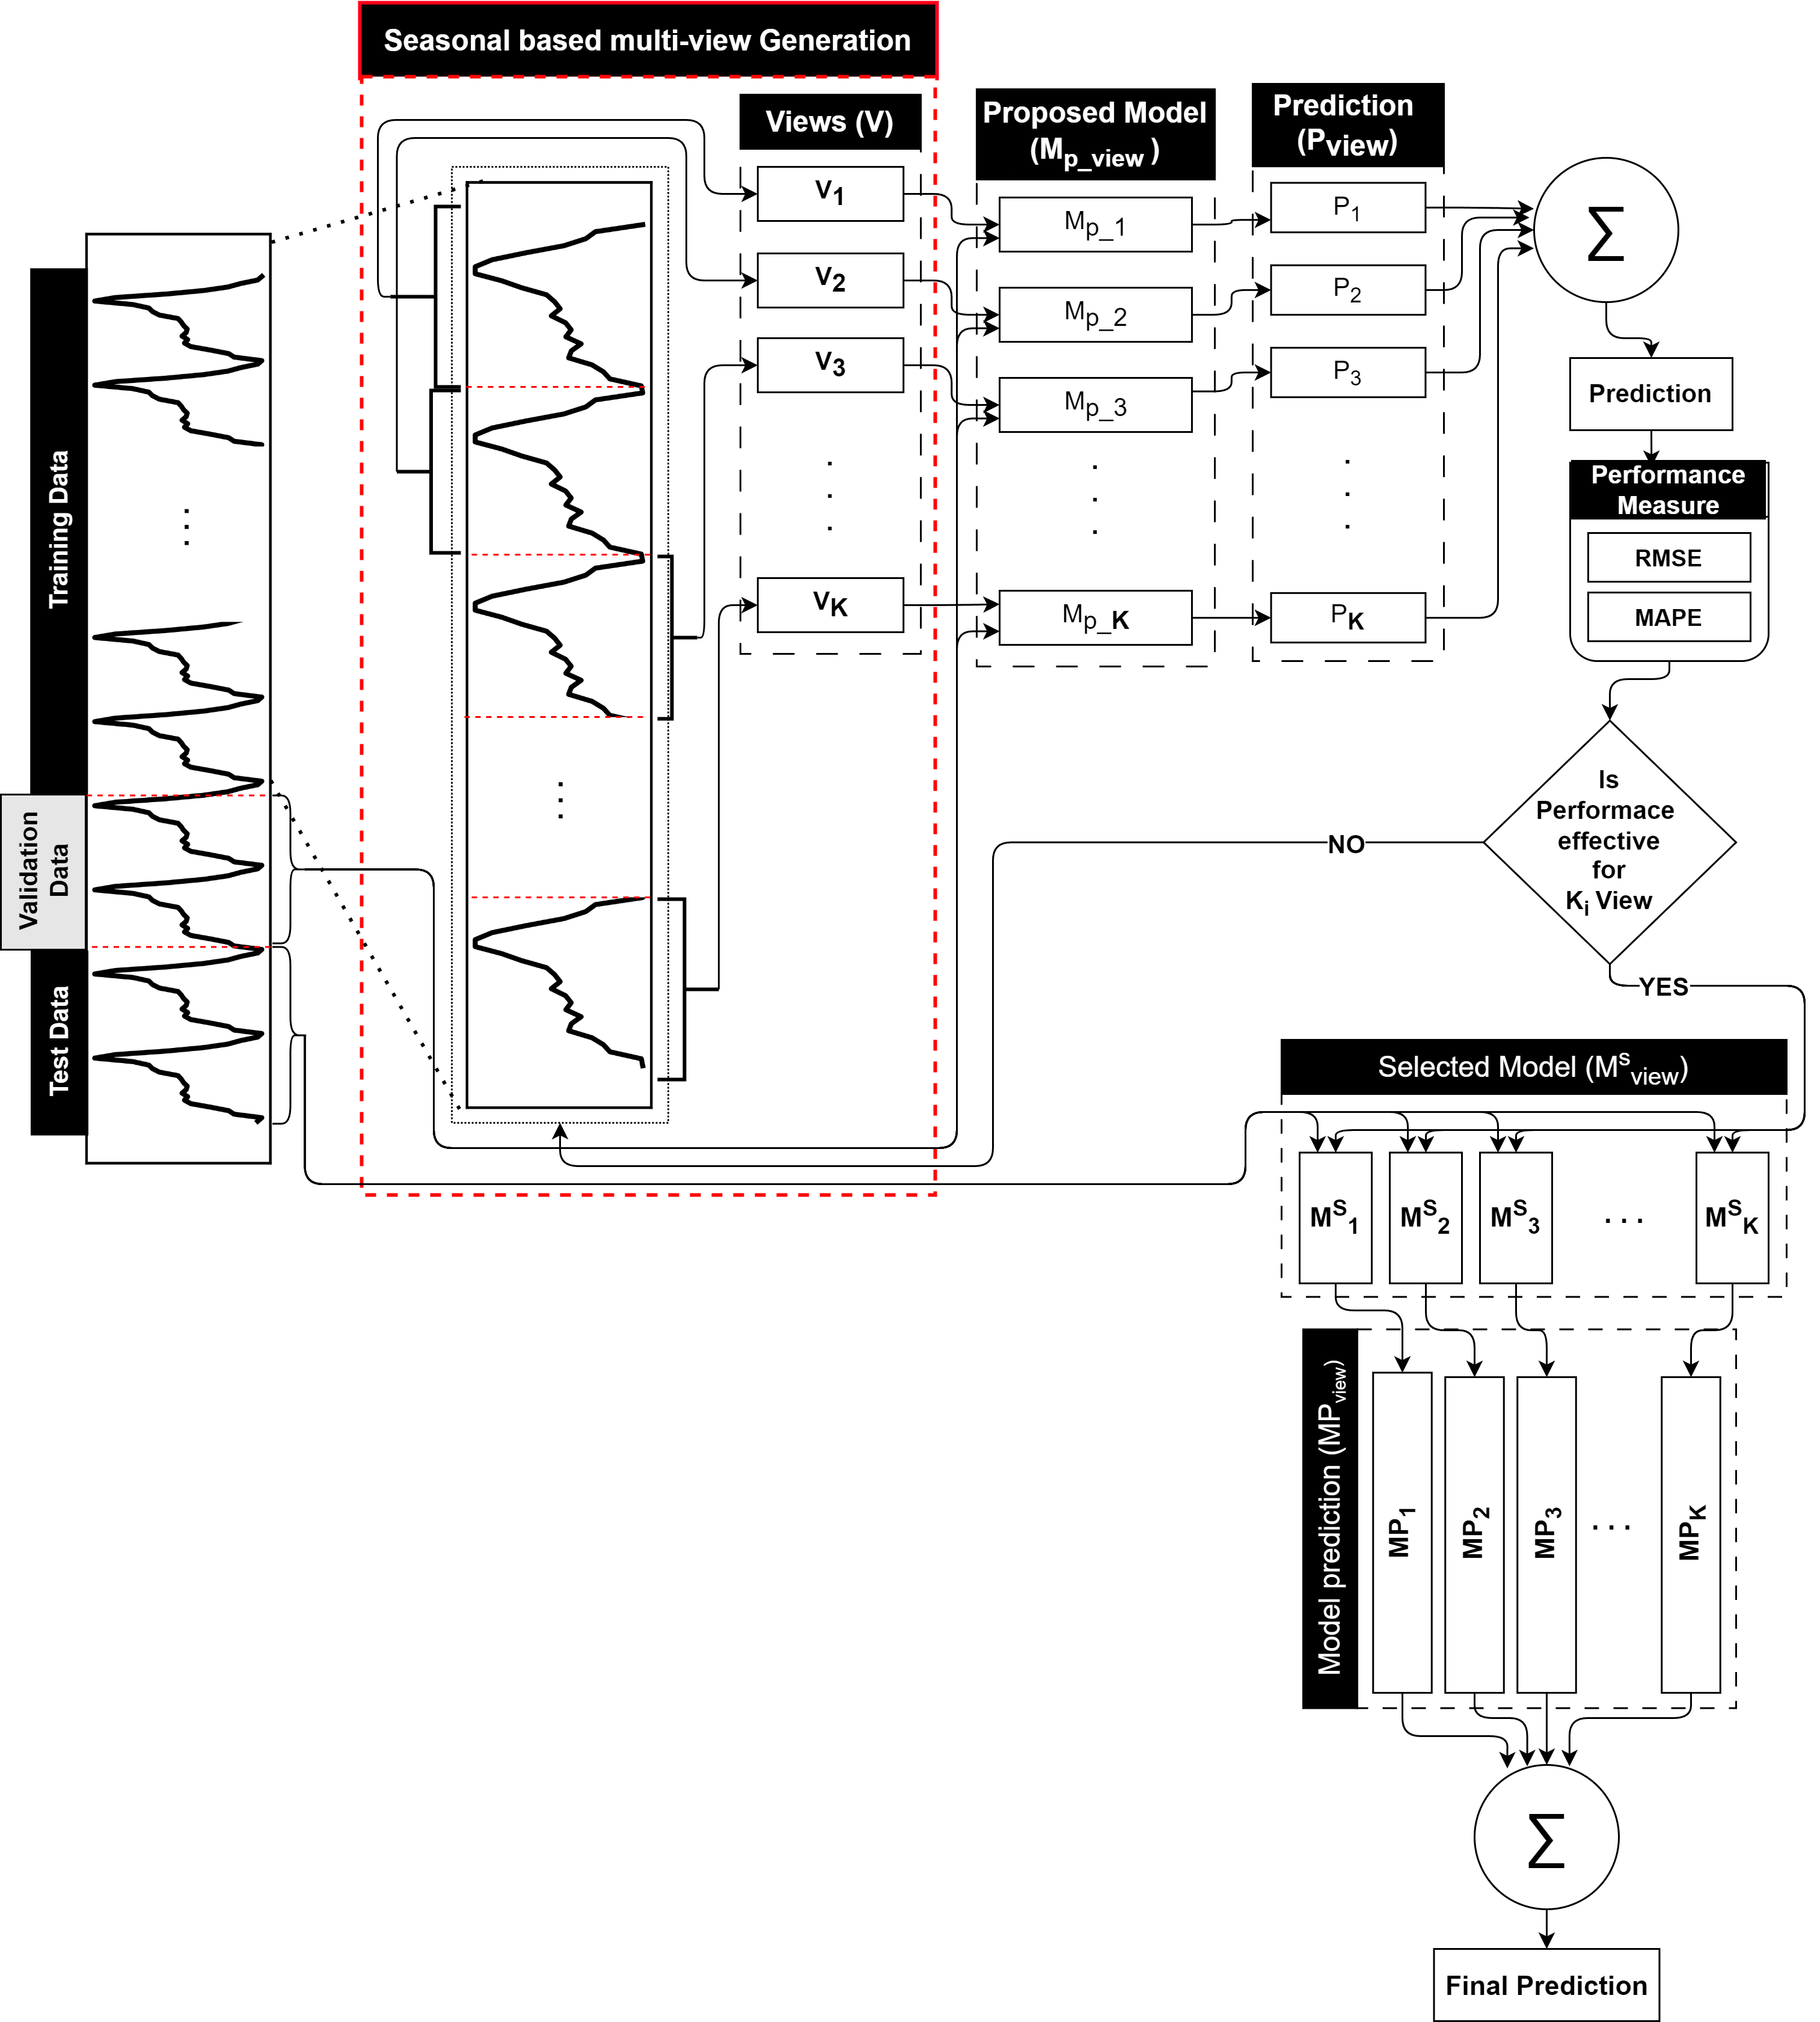
\includegraphics[scale=0.6]{img/MvS CNN-BiLSTM}
	  \caption{Flow diagram of proposed MultiView Stacked CNN-BiLSTM (MvS CNN-BiLSTM)}\label{Muticbilstm}
\end{figure*}


\subsection{Data:}

\begin{table*}[h!]
  \caption{Statistical exploratory data analyses $($EDA$)$ of 17 Time Series Datasets of polluted Indian cities based on $PM_{2.5}$ (\cite{bhawan2020central}).}
  \label{Eda1}
  
  \begin{tabular}{llccccccccc}
  \hline
  
  D.No. & DataSets & Year  & Samples &Mean &Std & Min &25\% &50\% &75\% & Max\\ \hline
  
 D1 &  BHIWADI          & 2017-2022  & 43394   & 108.03 & 79.76  & 0.02 & 55.22   & 97.32       & 135.36 & 999.99 \\ 
 D2 &  JODHPUR     & 2015-2022 &\textbf{61409} & 84.31 & 56.18 & 0.18 & 53.25   & 84.31 & 93.42   & 999.99 \\
 D3 &  SINGRAULI    & 2017-2022 & 43695   & 84.08 & 78.33 & 0.25 & 32.25   & 66          & 111.25  & 985    \\
 D4 &  ANKLESHWAR   & 2019-2022  & 33535     & 58.47 & 35.83 & 0.51 & 32.75   & 58.47 & 72.24   & 977.39 \\ 
 D5 &  LUDHIANA        & 2017-2022  & 49010  & 54.18 & 41.73 & 0.07 & 29.7    & 47.66       & 64.88   & 999.99 \\
 D6 &  DURGAPUR       & 2020-2022 & \textbf{17434}   & 71.67 & 46.20 & 0.33 & 37.47 & 62.05      & 98.03 & 565.41 \\ 
 D7 &  YAMUNA\_NAGAR  & 2019-2022 & 34299   & 77.86  & 52.31 & 0.1  & 43.8    & 69.91       & 94.28   & 930    \\
 D8 &  CHARKHI\_DADRI  & 2020-2022  & 24099   & 80.19 & 62.81 & 0.01 & 39.54  & 77.92       & 94.49  & 995.1  \\ 
 D9 &  JIND             & 2019-2022 & 34145 & 81.21 & 71.20 & 0.2  & 38.99   & 61.45       & 98.25   & 845.6  \\ 
 D10 &  KURUKSHETRA    & 2019-2022  & 34208 & 68.75& 53.80 & 0.46 & 33.33   & 56.38       & 87.56   & 962.7  \\ 
 D11 &  SONIPAT        & 2019-2022  & 34362  & 54.88 & 43.21  & 0.02 & 27.87   & 49.4        & 62.72   & 543.1  \\ 
 D12 &  DHARUHERA     & 2019-2022 & 34265 & 78.86 & 59.21 & 0.02 & 40.9    & 70.32       & 92.85   & 838.9  \\
 D13 &  AMBALA         & 2019-2022 & 34174 & 61.58 & 45.39 & 0.02 & 32.94   & 51.27       & 76.18 & 754.89 \\
 D14 &  HISAR          & 2019-2022 & 34143 & 86.22 & 71.02 & 0.63 & 42.62   & 69.33       & 102.89 & 999.99 \\ 
 D15 &  FATEHABAD      & 2019-2022 & 34160 & 63.01 & 60.46 & 0.07 & 32.63   & 49.01       & 72.5    & 999.99 \\
 D16 &  BULANDSHAHR  & 2018-2022 & 39869  & 90.53 & 85.08 & 0.25 & 34      & 63.75       & 120.25  & 985    \\ 
 D17 &  MUZAFFARNAGAR  & 2018-2022 & 38786 & 89.29 & 72.84  & 1    & 42.75   & 81.25       & 102.25  & 986    \\ \hline
 % \multicolumn{10}{l}{\textbf{Note:} first value of year show Data available from and second value of year show Data available till.}
  \end{tabular}
  \end{table*}
  
The Dataset in this study was collected from the Indian government portal CPCB (Central Pollution Control Board). These datasets contain univariate hourly data for 17 Indian cities, with most cities providing approximately 4 years' (show in Table \ref{Eda1}) . The table lists Bhiwadi, Jodhpur, Singrauli, Ankleshwar, Ludhiana, Durgapur, Yamuna Nagar, Charkhi Dadri, Jind, Kurukshetra, Sonipat, Dharuhera, Ambala, Hisar, Fatehabad, Bulandshahr, and Muzaffarnagar as the 17 cities from which data was collected shown on (Figure \ref{India map}) with Name , Latitude and Longitude . The Table \ref{Eda1} also provides information about the number of datapoint available in datasets and  highest number of datapoint in Jodhpur and lowest number of datapoint in Durgapur.

In Table \ref{Eda1} All the datasets are thoroughly analyzed based on several components such as Count,Min, Mean, Std,  25\%,Max , 75\%, and 50\%. The detailed description of the analysis is then sumarized for ease of understanding.
% Figure
\begin{figure*}[h!]
	\centering
		\includegraphics[scale=0.3]{img/india_map}
	  \caption{ Geograprical representation of polluted cities of India with their Latitude, Longitude and Name. }\label{India map}
\end{figure*}


\begin{comment}
% Please add the following required packages to your document preamble:
% \usepackage{graphicx}
\begin{table}[ht]
\caption{Data}
\label{undefined}
\begin{tabular}{llll}
\hline

DataSets       & Fast\_Day  & Last\_Day & No of Samples \\ \hline

BHIWADI        & 20-12-2017    & 02-12-2022  & 43394   \\
JODHPUR        & 01-12-2015     & 02-12-2022 & 61409   \\
SINGRAULI      & 08-12-2017     & 03-12-2022 & 43695   \\
ANKLESHWAR     & 04-02-2019     & 03-12-2022  & 33535   \\
LUDHIANA       & 01-05-2017    & 03-12-2022  & 49010   \\
DURGAPUR       & 06-12-2020   & 03-12-2022 & 17434   \\
YAMUNA\_NAGAR  & 03-01-2019   & 02-12-2022 & 34299   \\
CHARKHI\_DADRI & 03-03-2020    & 02-12-2022  & 24099   \\
JIND           & 10-01-2019      & 03-12-2022 & 34145   \\
KURUKSHETRA    & 07-01-2019      & 03-12-2022  & 34208   \\
SONIPAT        & 01-01-2019      & 02-12-2022  & 34362   \\
DHARUHERA      & 04-01-2019     & 02-12-2022 & 34265   \\
AMBALA         & 08-01-2019      & 02-12-2022 & 34174   \\
HISAR          & 10-01-2019      & 03-12-2022 & 34143   \\
FATEHABAD      & 09-01-2019      & 02-12-2022 & 34160   \\
BULANDSHAHR    & 16-05-2018      & 02-12-2022 & 39869   \\
MUZAFFARNAGAR  & 01-07-2018     & 03-12-2022 & 38786   \\ \hline
\end{tabular}
\end{table}
\end{comment}

\begin{itemize}

\item
\textbf{Preproccessing: }
Data preprocessing plays a critical role in machine learning projects as it ensures that the data is clean, consistent, and ready for analysis. Techniques like missing value imputation and min-max scaling facilitate data normalization and improve the effectiveness of machine learning algorithms by allowing them to learn from the data and make accurate predictions.
During the initial stage of data preprocessing, missing values are handled by replacing them with the means. The dataset is divided into 10 parts or chunks, and the mean is calculated for each chunk. Subsequently, the means of all the chunks are averaged together, as shown in.
\begin{equation} \label{equ:mean}
        x_i=\frac{\sum_{i=1}^{k} \left(\frac{D_{c_{i}}}{D_{s_{i}}} \right)}{k}
\end{equation}
 where $k=10$ \& $x_i$ is missing value in time series and $D_c$ represent chanks of Dataset. $D_s$ is the number of available samples in the dataset chunks represented by $D_c$. \\
Once the missing values have been imputed in the dataset using (equ(\ref{equ:mean})), then next step is to apply min-max scaling (equ(\ref{equ:minmax})). This technique ensures that univariate data is scaled to fall within the range of [0,1]. The scaling is achieved (equ(\ref{equ:minmax})):
\begin{equation}
        x_{norm, i}=\frac{x_i - \mu}{max(x)-min(x)}
        \label{equ:minmax}
    \end{equation}
where, $x_i$ is the $i^{th}$ data point and $\mu$ is mean of univariate data $min(x)$  and $max(x)$ denote the minimum values and maximum values in the univariate series.

The consistency is essential for comparing data across different datasets. Additionally, the scaling technique reduces the influence of outliers and enhances the data's robustness.


\item
\textbf{Decomposition and analysis:}

In Figure \ref{Eda} all subplot has been ploted on 480 Recent datapoints. Figure \ref{Eda} presents the graphical representation of the dataset, showcasing different categories like trend \&  seasonal. In rows 1, 4, and 7, the data is labeled as "Original." Rows 2, 5, and 8 correspond to the "Seasonal" category, while rows 3, 6, and 9 represent the "Trend" category. The last row combines all three categories, displaying "Original," "Seasonal," and "Trend" data in a single dataset. Each subplot within the graph has a specific dataset name, indicated in the legend.

The graph consists of five columns, each corresponding to a specific range of rows (1 to 3 , 3 to 6 and 6 to 9) from the dataset. The border color remains consistent across these columns, indicating that they belong to the same dataset. The legend provides clarity by associating the dataset name with its respective subplot, facilitating a comprehensive understanding of the data distribution and categories.

%By the Figure \ref{Eda} sesional every 24 Hour and per subplot has 20 numbers of sesional . in Graph sown some defrent type of trand present.

\begin{comment}
% Please add the following required packages to your document preamble:
% \usepackage{graphicx}
\begin{table}[ht]
\caption{Data}
\label{undefined}

\begin{tabular}{llllllll}
\hline

\textbf{DataSets}       &\textbf{Mean}  &\textbf{Std} &\textbf{ Min} &\textbf{25\%} &\textbf{50\%} &\textbf{75\%} & \textbf{Max}\\ \hline

\textbf{BHIWADI}         & 108.0337483 & 79.7575935  & 0.02 & 55.22   & 97.32       & 135.355 & 999.99 \\ 
\textbf{JODHPUR}       & 84.30884555 & 56.17507578 & 0.18 & 53.25   & 84.30884555 & 93.42   & 999.99 \\
\textbf{SINGRAULI}     & 84.07888484 & 78.32602035 & 0.25 & 32.25   & 66          & 111.25  & 985    \\
\textbf{ANKLESHWAR}     & 58.47126979 & 35.83229258 & 0.51 & 32.75   & 58.47126979 & 72.24   & 977.39 \\ 
\textbf{LUDHIANA}        & 54.18070537 & 41.72936492 & 0.07 & 29.7    & 47.66       & 64.88   & 999.99 \\
\textbf{DURGAPUR}      & 71.66516634 & 46.19819069 & 0.33 & 37.4725 & 62.045      & 98.0275 & 565.41 \\ 
\textbf{YAMUNA\_NAGAR}  & 77.8633741  & 52.30959419 & 0.1  & 43.8    & 69.91       & 94.28   & 930    \\
\textbf{CHARKHI\_DADRI}  & 80.19422853 & 62.81330763 & 0.01 & 39.535  & 77.92       & 94.485  & 995.1  \\ 
\textbf{JIND}           & 81.20790101 & 71.19703393 & 0.2  & 38.99   & 61.45       & 98.25   & 845.6  \\ 
\textbf{KURUKSHETRA}    & 68.75483661 & 53.80132654 & 0.46 & 33.33   & 56.38       & 87.56   & 962.7  \\ 
\textbf{SONIPAT}        & 54.88284717 & 43.2094932  & 0.02 & 27.87   & 49.4        & 62.72   & 543.1  \\ 
\textbf{DHARUHERA}      & 78.86179491 & 59.20936284 & 0.02 & 40.9    & 70.32       & 92.85   & 838.9  \\
\textbf{AMBALA}         & 61.58184731 & 45.39340564 & 0.02 & 32.94   & 51.27       & 76.1775 & 754.89 \\
\textbf{HISAR}          & 86.22030417 & 71.02050965 & 0.63 & 42.62   & 69.33       & 102.885 & 999.99 \\ 
\textbf{FATEHABAD}      & 63.01257933 & 60.46487543 & 0.07 & 32.63   & 49.01       & 72.5    & 999.99 \\
\textbf{BULANDSHAHR}   & 90.53344553 & 85.08059871 & 0.25 & 34      & 63.75       & 120.25  & 985    \\ 
\textbf{MUZAFFARNAGAR}  & 89.28704635 & 72.8395854  & 1    & 42.75   & 81.25       & 102.25  & 986    \\ \hline
\end{tabular}
\end{table}
\end{comment}
\begin{figure*}[h!]
  \centering
  \subfigure{\includegraphics[scale=0.208]{img/eda1}}
  \subfigure{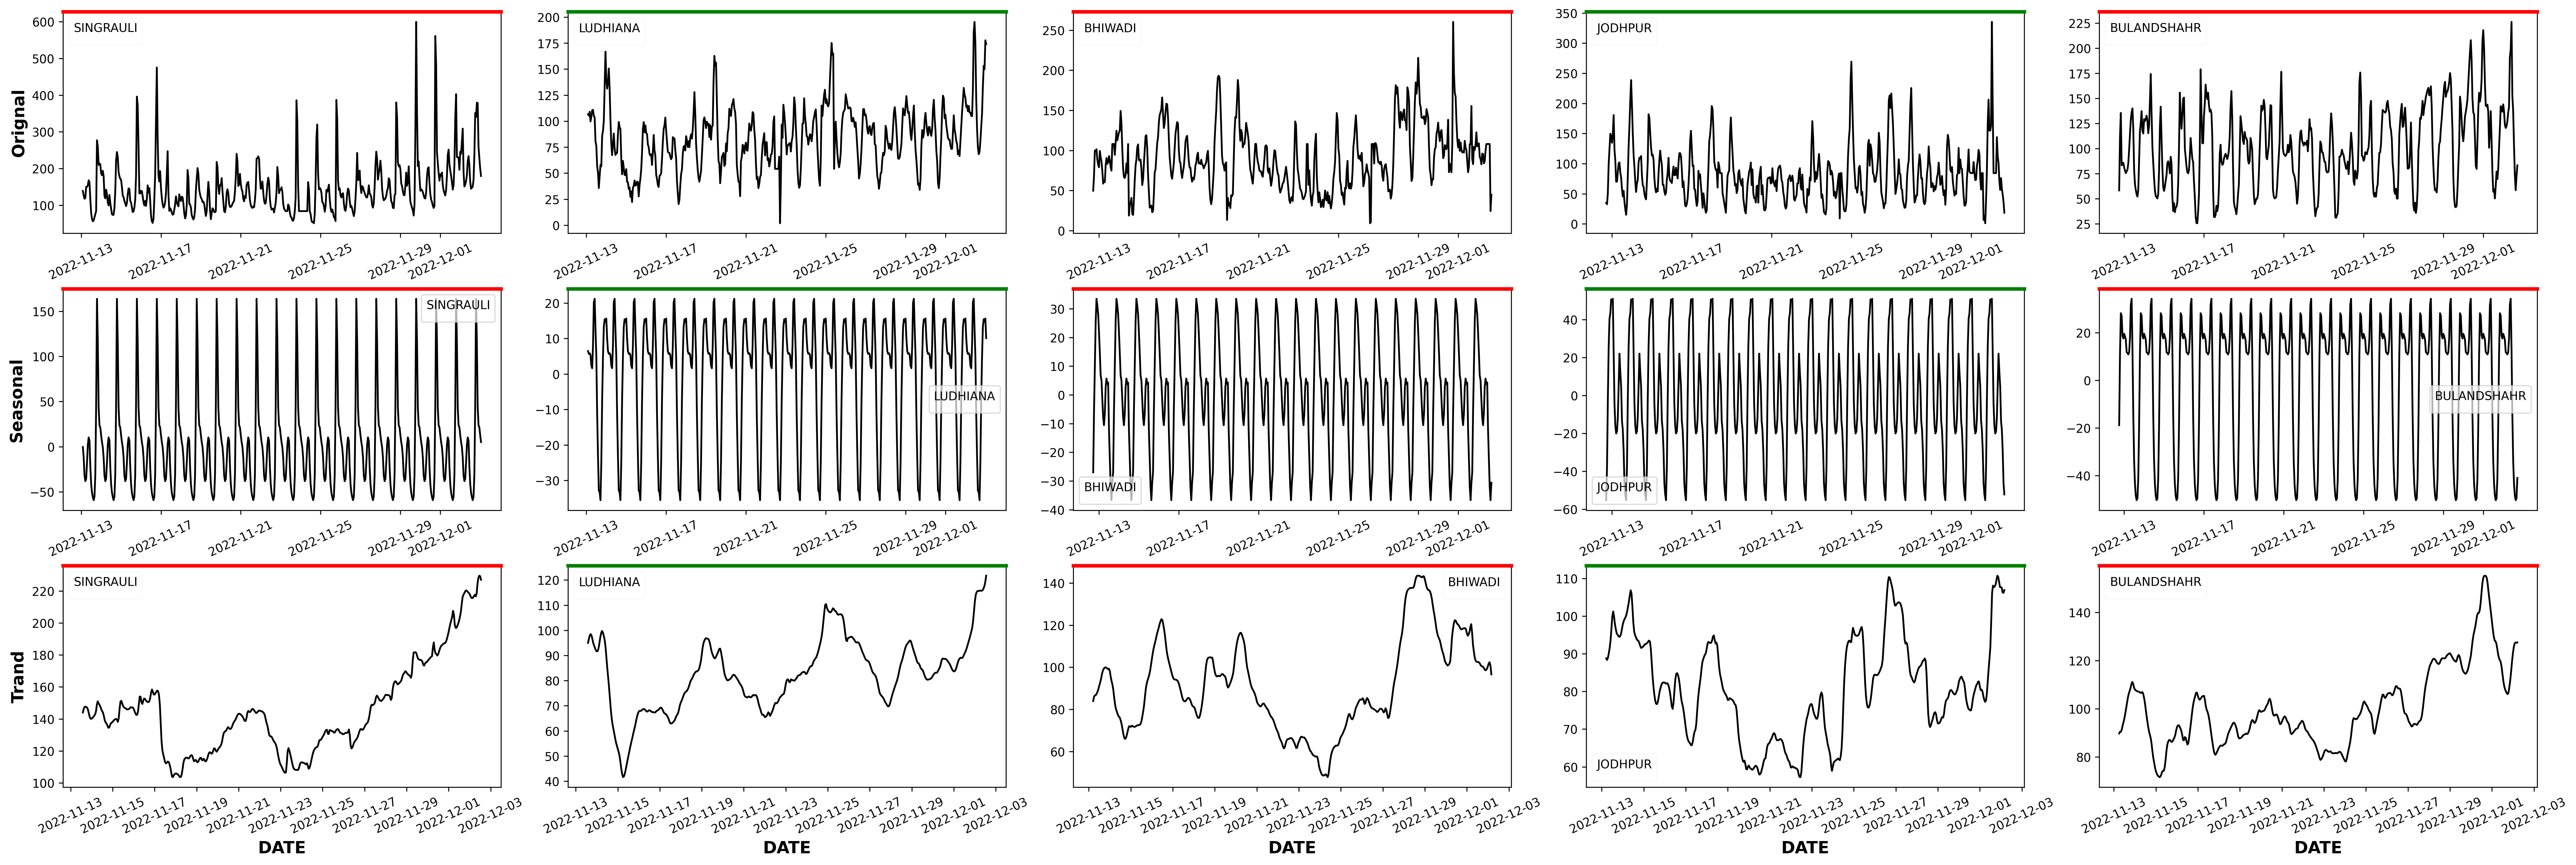
\includegraphics[scale=0.208]{img/eda2}}
  \subfigure{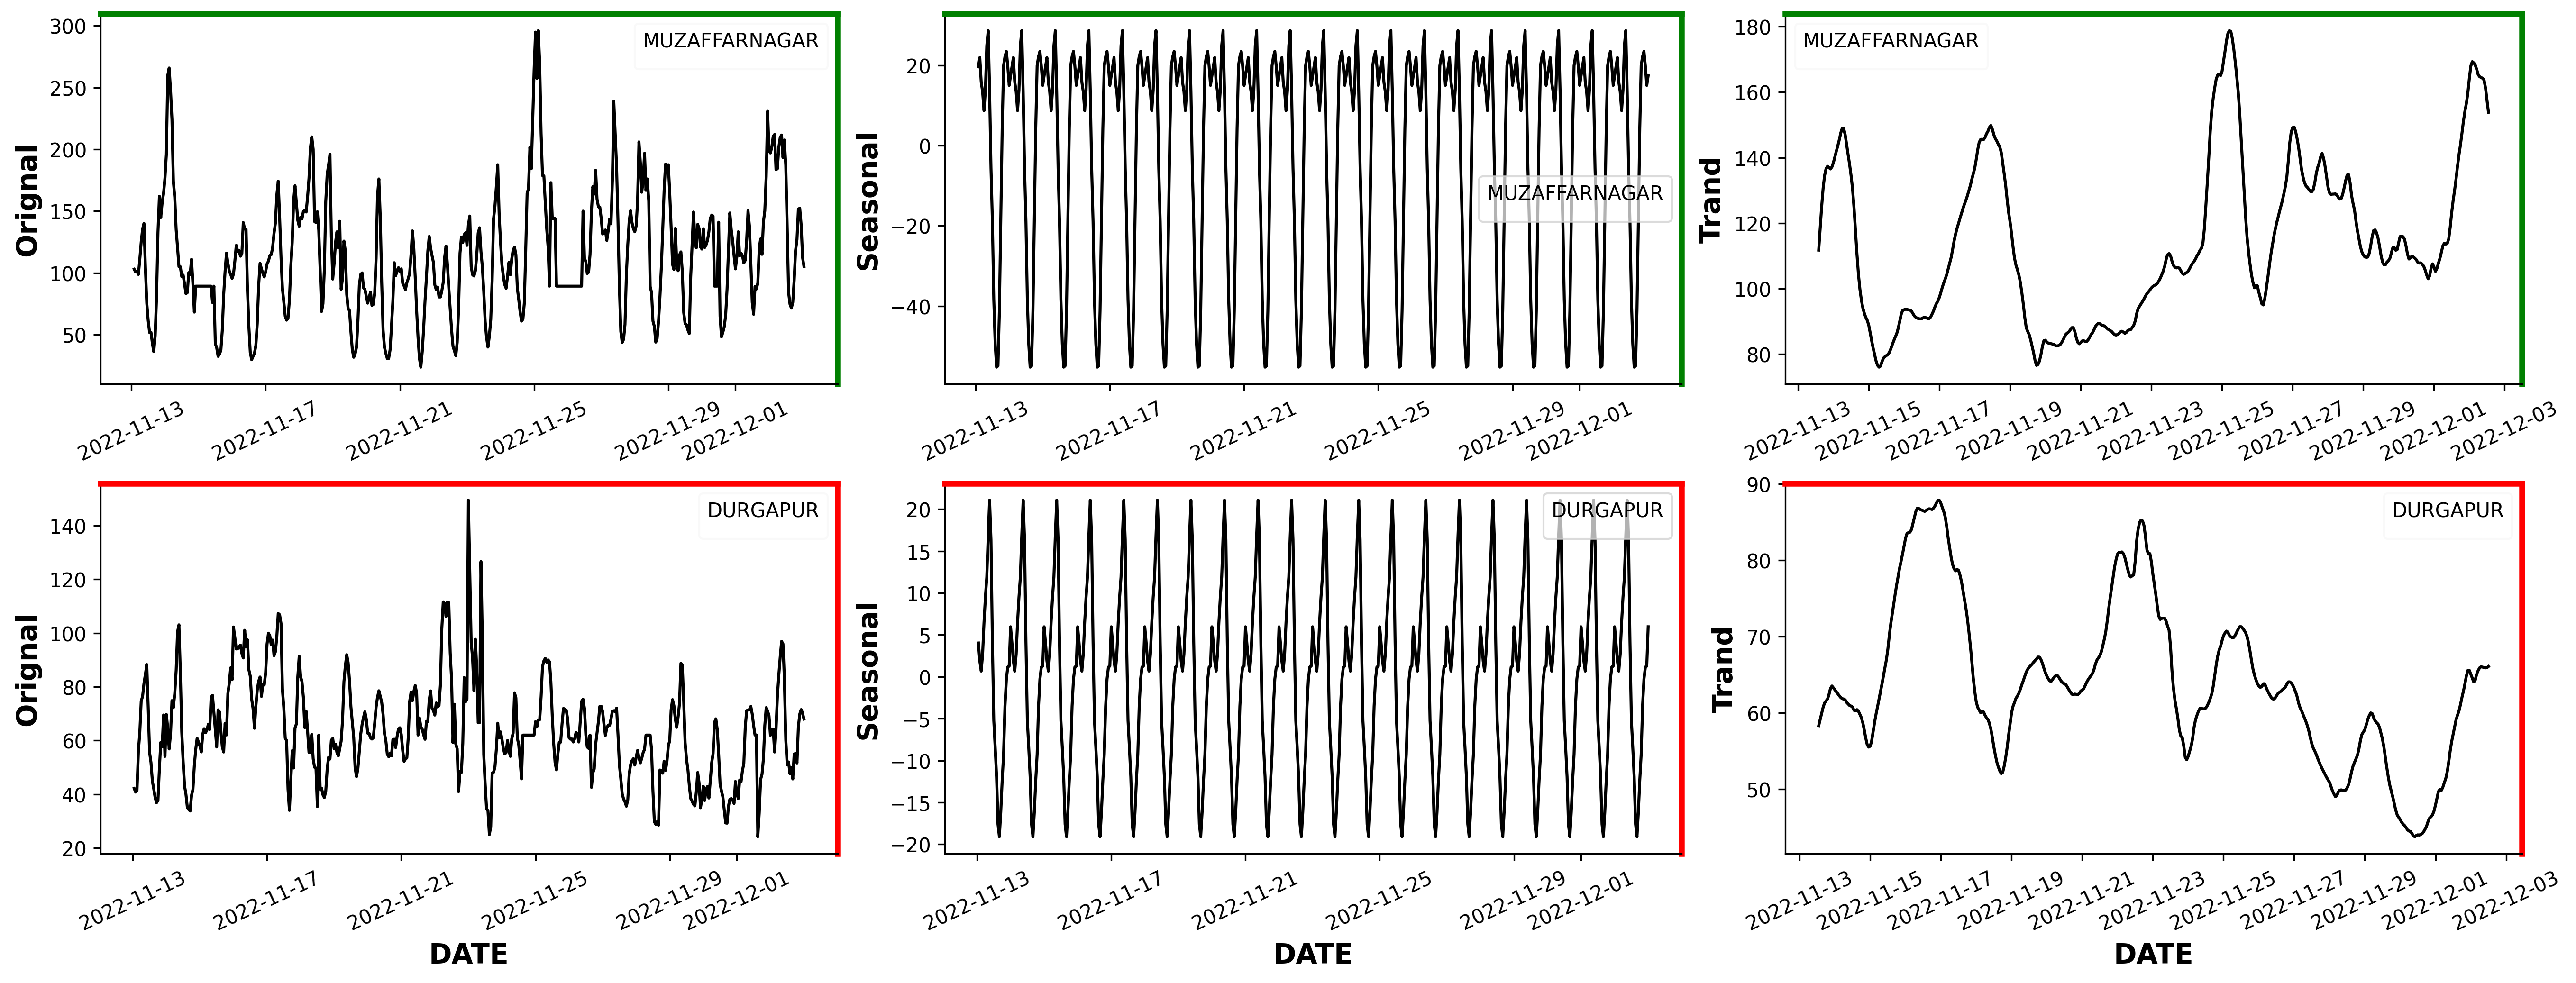
\includegraphics[scale=0.208]{img/eda3}}
  \caption{Decomposition of 17 dataSets based on trand, sesiosnal along with original dataset.}
  \label{Eda}
\end{figure*}
Figure \ref{Eda} illustrates the seasonal variations in the dataset with a frequency of every 24 hours. Each subplot within the graph contains 20 data points representing the seasonal pattern. Additionally, the graph showcases various types of trends present in the data. These trends may include upward trends, downward trends, or fluctuating trends over time. The combination of seasonal variations and diverse trends provides valuable insights into the underlying patterns and behaviors of the dataset.
\end{itemize}




\begin{comment}
  % Figure
\begin{figure}[ht]
	\centering
		\includegraphics[scale=0.208]{img/eda1}
	  \caption{Original,Sesisonality and Trand for 10 DataSets 480 datapoints pick for Graph.Same bodder color and type of bodder indecate same dataset colums by. $1^{st}$ and $4^{th}$ row show original data , $2^{nd}$ and $5^{th}$ row show Sesisonality and $3^{rd}$ and $6^{th}$ row show Trend. }\label{o_r_t1}
\end{figure}
% Figure
\begin{figure}[ht]
	\centering
		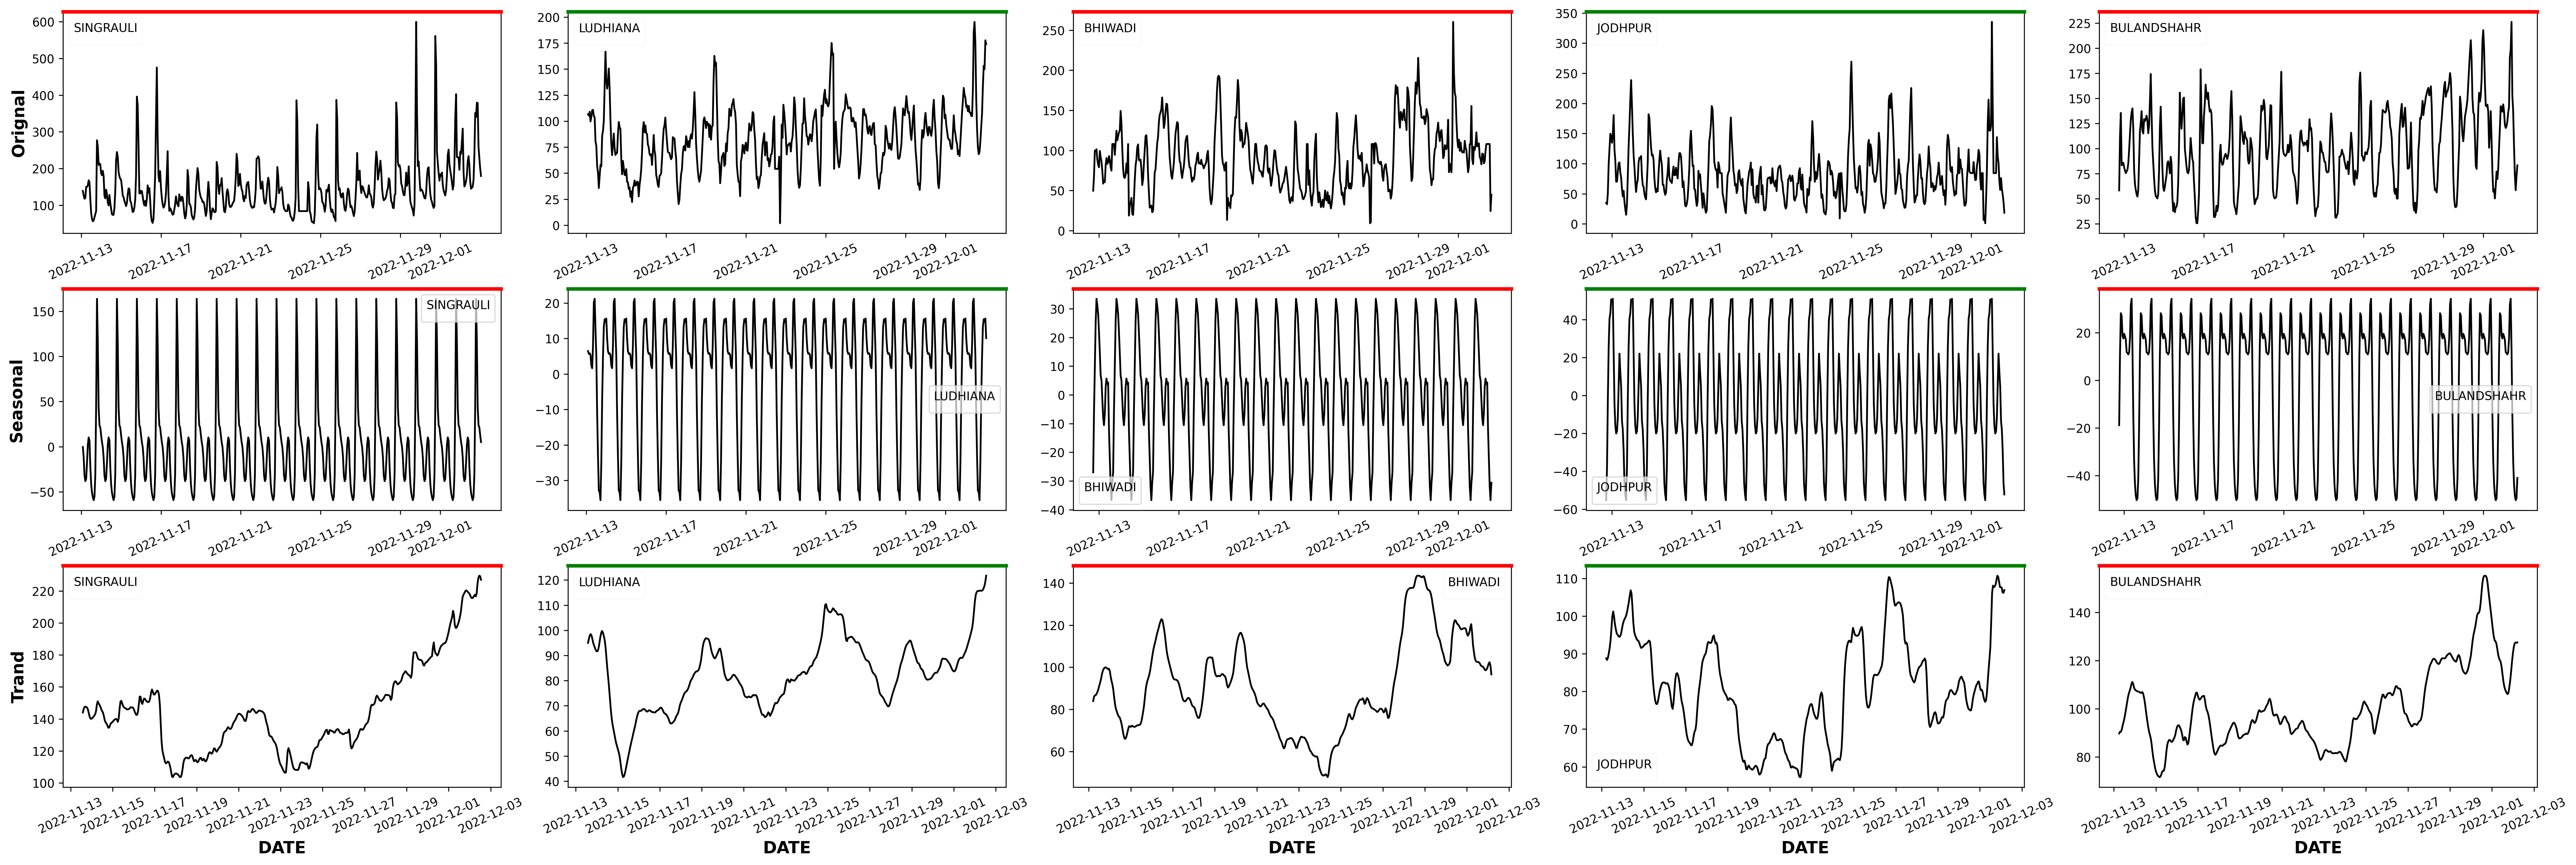
\includegraphics[scale=0.208]{img/eda2}
	  \caption{Original,Sesisonality and Trand for 5 DataSets 480 datapoints pick for Graph.Same bodder color and type of bodder indecate same dataset colums by. $1^{st}$ row show original data , $2^{nd}$  row show Sesisonality and $3^{rd}$ row show Trend.}\label{o_r_t2}
\end{figure}
% Figure
\begin{figure}[ht]
	\centering
		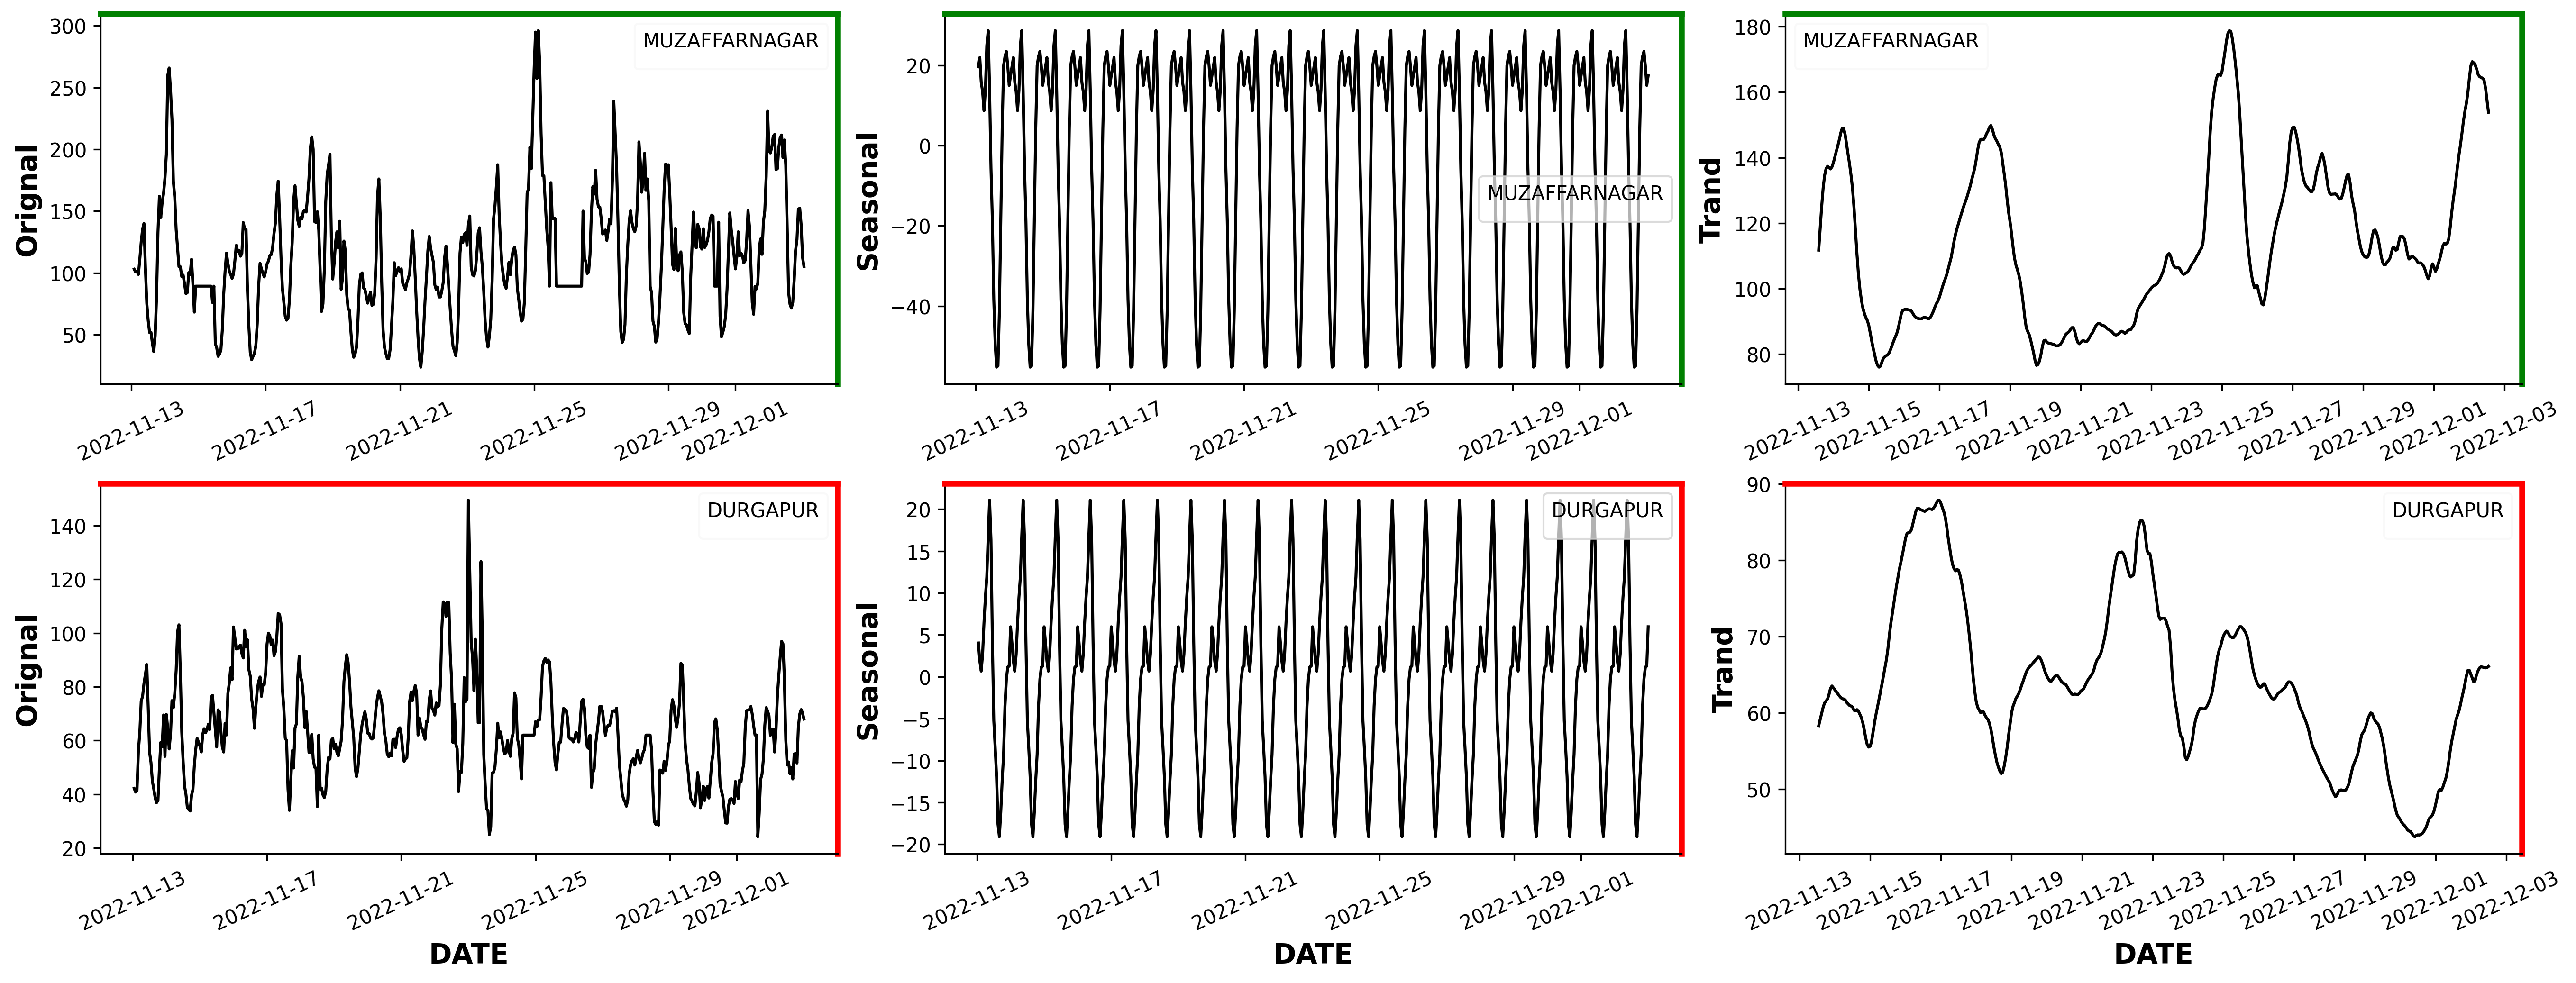
\includegraphics[scale=0.208]{img/eda3}
	  \caption{Original,Sesisonality and Trand for 5 DataSets 480 datapoints pick for Graph.}\label{o_r_t3}
\end{figure}
\end{comment}



\subsection{Deep learning models}
\subsubsection{Convolutional Neural Network (CNN)}
A CNN is an essential neural network utilized extensively for analyzing time series and processing signals. Unlike standard fully connected neural networks, which process input as vectors, 1D CNNs extract local features using convolution operations using a sliding window technique. They're made to operate with one-dimensional signals like audio or time series sensor readings. In Figure \ref{CNN} (\cite{chaerun2021comparative}) 1D CNN, multiple filters are employed to extract various features from the input signal. These filters slide over the input, capturing local patterns and representations The convolutional layer output is then downsampled using pooling layers, reducing the dimension of the data and preventing overfitting. The network may also include fully connected layers that perform tasks like as classification or regression using the retrieved features.

The simplicity of the 1D CNN (\cite{kiranyaz20211d}) architecture lies in its effectiveness in extracting features from one-dimensional signals. The sliding window approach allows the network to focus on local details and extract relevant information effectively. Furthermore, the convolutional process reduces the number of parameters, resulting in a more computationally efficient network. Pooling layers help in generalization by decreasing output complexity, resulting in higher performance on previously unknown data. 1D CNNs are versatile and effective in a range of domains since they can examine historical data and extract relevant characteristics. They've shown to be incredibly effective in applications such as speech recognition (\cite{rusnac2022cnn,wang2019end}), audio categorization (\cite{ashraf2022role,hu2020device}), and sensor data processing (\cite{kattenborn2021review,sun2019classification}). Overall, 1D CNNs are powerful tools for collecting features from one-dimensional data, providing important insights, and paving the way for advances in signal processing and time series analysis.

\begin{figure*}[h!]
  \centering
    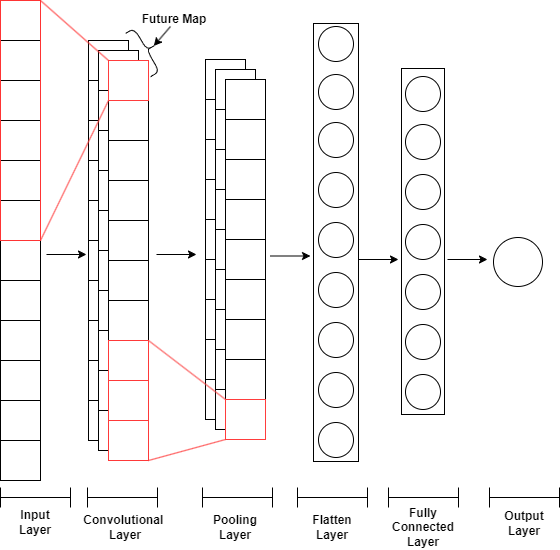
\includegraphics[scale=.5]{img/cnn}
    \caption{Traditional architecture of $1D-CNN$}\label{CNN}
\end{figure*}

1D CNN use a set of learnable filters (or kernels) of length k to carry out the convolution operation. This operation involves computing the dot product between the filter and a k-length window sliding over the input sequence x with length L, then new sequence of feature map generated as outcome.

Denoting the set of filters as $F$ and the output feature map at position $i$ as $h_i$, we can express the output feature map $h$ as follows:
\begin{equation}\label{equ:cnn}
        h_i = \sigma \left (\sum_{j=1}^{k}F_{j}.x_{i+j-1}+b \right)
\end{equation}
where, $F_j$ represents the $j^{th}$ filter in the set of filters $F$, $x_{i+j-1}$ is the value of the input sequence $x$ at position $(i+j-1)$, $\sigma$ is the activation function (such as ReLU or sigmoid), and $b$ is the bias term.

\subsubsection{Gated Recurrent Unit (GRU)}
The GRU is a specialized recurrent neural network architecture designed for managing sequential data input  (\cite{chung2014empirical}) and unique proposal was put forth as a substitute for the well-liked LSTM network. These gating mechanisms selectively update the hidden state, allowing GRU to effectively capture dependencies in sequential data. GRU has found use in an array of areas, including speech recognition (\cite{shewalkar2019performance,yuan2018auxiliary}), natural language processing (\cite{cascianelli2018full,wang2020feature}), and picture recognition (\cite{subramanian2022integrated}), due to its gating mechanisms and ability to handle sequential dependencies. Its capabilities make it a powerful tool for modeling and understanding sequential data, providing valuable insights and improved performance in numerous tasks. GRU network based on gates and states are shown in equ(\ref{up Gru}) to equ(\ref{hid gru}):\\

 
\begin{equation} \label{up Gru}
  Update Gate : z_t= \sigma(W_{z}\cdot \left[ h_{t-1},x_t \right]+b_z )
\end{equation}

\begin{equation}\label{r gru}
  Reset Gate : r_t=\sigma (W_{r}\cdot \left[ h_{t-1},x_t \right]+b_r )
\end{equation}

\begin{equation} \label{can gru}
  Candidate activation : \tilde{h_t}=tanh(W_h \cdot \left[ r_t \odot h_{t-1},x_t \right]+b_h)
\end{equation}

\begin{equation} \label{hid gru}
  Hidden State :  h_t=(1-z_t) \odot h_{t-1}+z_t \odot \tilde{h_t}
\end{equation}


\begin{comment}
At time step t, the hidden state is represented by $h_t$​, the input is represented by $x_t$​, and the update and reset gates are represented by $z_t$ and $r_t$​ respectively. The refresh entryway directs the amount of the past covered state to keep for the present time step, while the reset entryway controls the amount of the past covered state to overlook. 
The candidate activation, $\tilde{h_t}$​, represents new information that could be added to the hidden state. The sigmoid activation function, $\sigma$ and element-wise multiplication represented by $\odot$ are used. Weight matrices $W_z$,$W_r$,$W_h$ and bias vectors $b_z$,$b_r$,$b_h$​ are also utilized. The GRU's update and reset gates allow it to learn when to update the hidden state and what information to forget, making it particularly useful for modeling sequential data with long-range dependencies.
\end{comment}
where, time step t, the hidden state is represented by $ h_t $ , the input is represented by $ x_t $ , and the update and reset gates are
represented by $ x_t $ and $ r_t$ respectively. The refresh entryway directs the amount of the past covered state to keep for the present time step, while the reset entryway controls the amount of the past covered state to overlook.The candidate activation $\tilde{h_t}$ ,represents new information that could be added to the hidden state.The sigmoid activation function $ \sigma $ and element-wise multiplication represented by $\odot$ are used.Weight matrices $ W_z $, $ W_r $, $ W_h $ and bias vectors $ b_z $, $ b_r $, $ b_h $ are also utilized. The GRU's update and reset gates allow it to learn when to update the hidden state and what information to forget, making it particularly useful for modeling sequential data with long-range dependencies.
\subsubsection{Recurrent Neural Network (RNN)}
RNN is an ANN that utilizes the outcome of the preceding measure as a contribution to the present step. Forecasting the succeeding phrase in a statement is not a strong suit of RNNs because their Memory State, also recognized as the hidden layer, does not preserve any data about preceding words. It stores the previous input given to the network, which goes a long way in ensuring accurate predictions. The RNN technique employs identical parameters for every input, leading to it executing the same function on every hidden layer to obtain the end results. significantly reduces the complexity of parameters, unlike other neural networks, making it a popular choice among researchers and developers. The elegance of RNN rests in its capacity to recall prior inputs, rendering it a valuable instrument in creating predictions that demand context. Ordinarily, profound learning has been exhibited to be a game-changer in the area of AI and ML, and it will without a doubt persist to be an essential instrument in the coming years.

Recurrent Neural Network (RNN) model are input \& output to hidden state can be written as equ(\ref{equ:ih rnn}) \& equ(\ref{equ:h rnn}) respectiveely:

  \begin{equation} \label{equ:ih rnn}
    Input to Hidden State: h_t= \psi (W_{hx} \cdot x_t + W_{hh} \cdot h_{t-1} +b_h)
  \end{equation}
  \begin{equation} \label{equ:h rnn}
    Hidden State to Output: y_t=W_{yh}\cdot h_t+b_y
  \end{equation}
where, $h_t $ is the hidden state at time step $t$, $x_t$ is input at $t$ step of time, $y_t$ is output at t step of time, $W_{hx} $ is a weight matrix that links the input to the concealed state, $W_{hh}$ is the weighted matrix that connects the state that is hidden at time step $t-1$ with the hidden value at time step t, $W_{yh}$ is a weighted matrix that links the state that is hidden to the output, $b_h$ and $b_y$ are biassed terms for both the state that is hidden and the output and $\psi (\cdot)$ is a function of activation applied to the concealed state element by element.


\subsubsection{Long-Short-Term Memory (LSTM)}
LSTMs are a specialized type of RNN designed to handle sequential data. They excel at learning long-term dependencies, making them suitable for language translation, speech recognition, and time series forecasting. The utilization of the memory cell and three gates facilitates the capability of LSTMs to learn intricate patterns in data by selectively retaining and discarding information. Deep LSTM networks, achieved by stacking LSTMs, are particularly useful for tasks like speech recognition (\cite{soltau2016neural,jo2020approximate}) and natural language processing (\cite{wang2015learning,nammous2019natural}). Hochreiter and Schmidhuber  (\cite{hochreiter1997long}) developed LSTMs to overcome the long-term dependency issue in traditional RNNs. LSTMs are widely used in processing (\cite{sahin2018nonuniformly}), prediction (\cite{gers2000learning}), and classification (\cite{zhou2015c,karim2017lstm}) of temporal data, and when combined with CNNs, they efficiently analyze images (\cite{li2019cnn,rajendran2020land,islam2020combined}) and videos (\cite{ullah2017action,li2020classifying,gao2017video,bin2018describing}) by extracting spatial and temporal features. LSTMs are an effective instrument for analyzing sequential data and can be incorporated with other neural network structures to accomplish more complex objectives.
The LSTM architecture related gates and states are shown in equ(\ref{lstm i}) to equ(\ref{lstm h})

  \begin{equation} \label{lstm i}
    Input Gate : i_t=\sigma (W_{xi}\cdot x_t+W_{hi}\cdot h_{t-1}+b_i)
  \end{equation}
 
  \begin{equation}\label{lstm f}
    Forget Gate : f_t= \sigma(W_{xf}\cdot x_t +W_{hf}\cdot h_{t-1}+b_f)
  \end{equation}

  \begin{equation}\label{lstm c}
    Candidate Hidden State :  g_t=than(W_{xg}\cdot x_t+W_{hg}\cdot h_{t-1} +b_g)
  \end{equation}

  \begin{equation}\label{lstm ce}
    Cell State : C_t=f_t \odot C_{t-1}+i_t \odot g_t
  \end{equation}

  \begin{equation}\label{lstm o}
    Output Gate : o_\sigma(W_{xo}\cdot x_t +W_{ho}\cdot h_{t-1}+b_o)
  \end{equation}

  \begin{equation} \label{lstm h}
    Hidden State :  h_t=o_t \odot tanh(C_t)
  \end{equation}
whare, $h_t$ at time step, is the concealed condition (also known as a hidden representations), $x_t$  is the time step input, $C_t$  is the condition of the cell at time step $t$, serving as the LSTM's long-term memory, $\sigma$ Its sigmoid activation function , The tangent hyperbolic activation function is denoted by tanh, $\odot$ represents element-by-element multiplication, $W_{xi}$, $W_{hi}$, $W_{xj}$, $W_{hf}$, $W_{xg}$, $W_{hg}$, $W_{xo}$, $W_{ho}$ are the matrices of that will be taught throughout training and $b_i$, $b_f$, $b_g$, $b_o$ are slanted terms.


\subsubsection{Bi-directional Long Short Term Memory (BiLSTM)}
BiLSTM is a type of human stupidity designed to process sequential data in neither forward nor backward directions. The plan uses dual LSTM layers for both forward and backward processing concurrently, enabling it to grasp the context from both previous and upcoming time steps. Therefore, the network cannot identify any relationships in either direction, making it a disadvantage for tasks such as speech recognition and language translation. By providing a broader perspective of the input sequence, BiLSTMs can improve the performance in tasks requiring contextual understanding. These forms are remarkable for long-term dependencies and are commonly utilized in profound learning projects.

\begin{figure*}[h!]
  \centering
  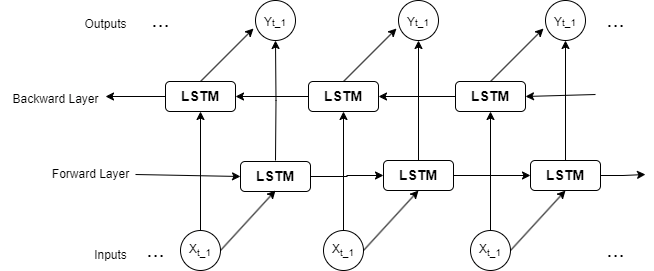
\includegraphics[scale=0.6]{img/Bilstm}
  \caption{Architecture of BiLSTM (\cite{article})} \label{Bilstm}
\end{figure*}



BiLSTM network architecture gates and states are shown below from equ(\ref{bi i}) to equ(\ref{bi h})
\begin{itemize}
  \item  Forward LSTM:\\

    \begin{equation} \label{bi i}
      Input Gate : i_t^f = \sigma(W_{xi}^f \cdot x_t + W_{hi}^f \cdot h_{t-1}^f + W_{ci}^f \cdot c_{t-1}^f + b_i^f)
    \end{equation}

    \begin{equation}
      Forget Gate : f_t^f = \sigma(W_{xf}^f \cdot x_t + W_{hf}^f \cdot h_{t-1}^f + W_{cf}^f \cdot c_{t-1}^f + b_f^f) 
    \end{equation}

    \begin{equation}
      Candidate Hidden State :  g_t^f = \text{tanh}(W_{xg}^f \cdot x_t + W_{hg}^f \cdot h_{t-1}^f + b_g^f)
    \end{equation}

    \begin{equation}
      Cell State : c_t^f = f_t^f \odot c_{t-1}^f + i_t^f \odot g_t^f
    \end{equation}

    \begin{equation}
      Output Gate : o_t^f = \sigma(W_{xo}^f \cdot x_t + W_{ho}^f \cdot h_{t-1}^f + W_{co}^f \cdot c_t^f + b_o^f)
    \end{equation}

    \begin{equation} \label{bi h}
      Hidden State :  h_t^f = o_t^f \odot \text{tanh}(c_t^f) 
    \end{equation}

  \item Backward LSTM:
  The formulas for the rear LSTM are similar to those of the forward LSTM but with different sets of weights and biases. The subscript "b" is used to denote the backward direction (e.g., \(W_{xi}^b\) is the weight matrix for the input gate in the backward LSTM). The BiLSTM combines the forward and backward hidden states to form the final output. The output \(y_t\) at time step \(t\) is typically computed using a combination of both forward and backward hidden states. The exact approach for combining the two directions (e.g., concatenation, addition, etc.) depends on the specific task and model architecture.
\end{itemize}




\subsection{ Performance Measures}
\subsubsection{Root Mean Square Error (RMSE) }
The RMSE is hardly ever utilized as a standard for assessing the precision of a regression model. The computation of the root mean square of discrepancies between projected and factual figures can facilitate identifying the divergence between them, while keeping the units of measurement consistent with the data. This provides valuable insight into the model's effectiveness. A lower RMSE digit suggests superior model performance, while an increased RMSE value indicates substandard model performance. The RMSE equ(\ref{rmsee}) useul metric for regression models by effectively evaluating the model's accuracy, as it quantifies the discrepancy between projected and actual values in the same unit as the data.Through analysis of the RMSE score, experts can evaluate the model's efficacy and implement necessary tweaks to enhance its precision. As a final point, the RMSE is a crucial statistic for evaluating the accuracy of regression models, and its usage is essential in industries that heavily depend on data science, finance, and engineering.



\begin{equation} \label{rmsee}
RMSE=\sqrt{\frac{\sum_{i=1}^{n}(y_{i}-\hat{y_{i}})^2}{n}}
\end{equation}
where $n$ represents the number of times that the summation iteration occurs, \begin{math} y_{i} \end{math} denotes the actual value, and \begin{math}\hat{y_{i}}\end{math} represents the forecast value.




\subsubsection{ Mean Absolute Percentage Error (MAPE)}
A popular metric for judging the efficiency of regression models is MAPE. Essentially, it measures the percentage of variance between predicted and actual results and averages these discrepancies. MAPE can be computed by finding the average of the absolute percentage errors between the expected and actual values, such as equ(\ref{mapee})
\begin{equation} \label{mapee}
MAPE=\frac{1}{n}\sum_{i=1}^{n} \left | \frac{y_{i}-\hat{y_{i}}}{y_{i}} \right |
\end{equation}
where $n$ represents the number of times that the summation iteration occurs, \begin{math} y_{i} \end{math} denotes the Actual value, and \begin{math}\hat{y_{i}}\end{math} represents the forecast value.

MAPE is utilized to determine the average percentage discrepancy between the projected and observed values. In the world of business and finance, it is a common practice to assess the precision of forecasts or predictions using this technique. Industries utilize MAPE to compute the mean percentage deviation between anticipated and actual values, where a lower value suggests better model performance and a higher value suggests poorer performance. However, MAPE can cause division by zero errors or very large percentage errors when the actual numbers are close to zero.




\subsection{Model Devlopment}
\subsubsection{Proposed Multi-view Stacked CNN-BiLSTM (MvS CNN-BiLSTM)}
% Figure
\begin{figure*}[h!]
	\centering
		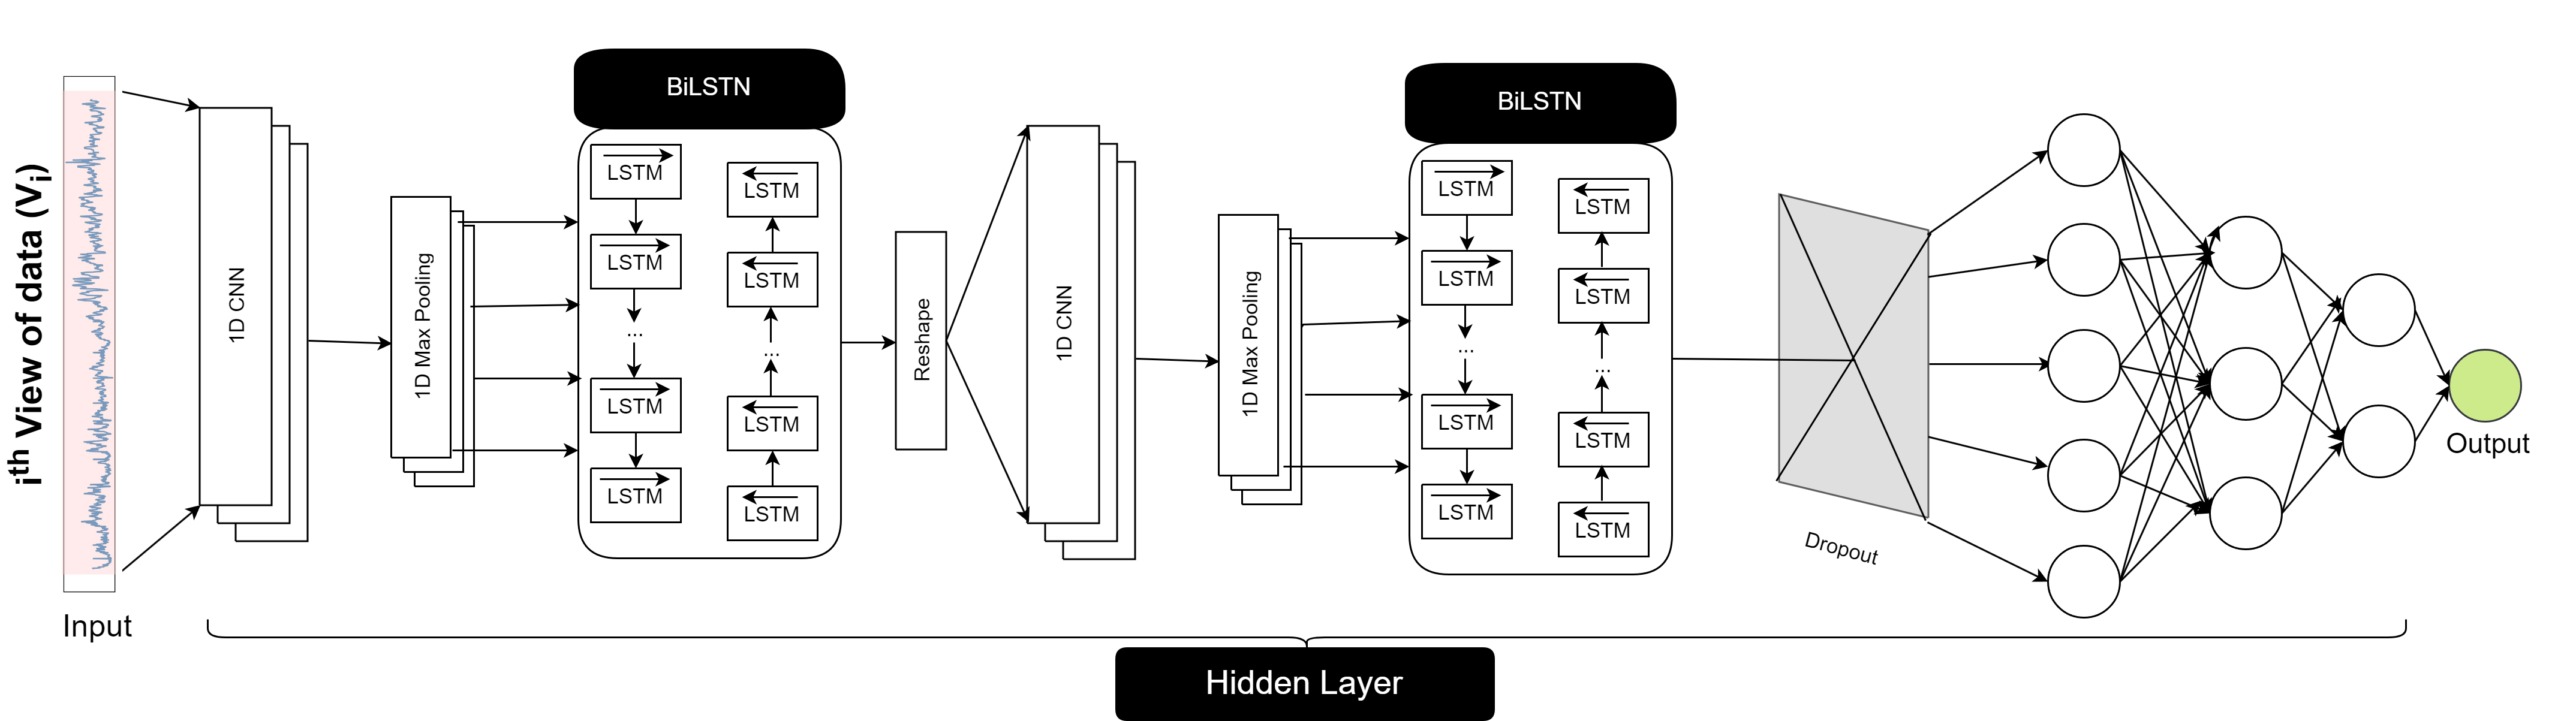
\includegraphics[scale=0.5]{img/Prpose}
	  \caption{Architecture of Stacked CNN-BiLSTM}\label{prosed_cnn-bilstm}
\end{figure*}

The model consists of various layers, starting with a 1D Convolutional layer with 128 filters , followed by a MaxPooling layer for downsampling. Next, a Bidirectional LSTM layer with 64 units and 'relu' activation is applied, returning only the last output. To reshape the output, a Reshape layer is introduced, another 1D Convolutional layer with 32 filters is utilized, followed by another MaxPooling layer. Another Bidirectional LSTM layer with 32 units and 'relu' activation is added, again returning only the last output. To prevent overfitting, a Dropout layer with a rate of 0.2 is introduced before the final Dense layer, which contains a single neuron for regression predictions.The model is given the name 'stacked CNN-BiLSTM'.

\subsubsection{Implamentation setup and parameters settings}
The various python packages are utilized to implement both the proposed and baseline models. These assortments incorporate Keras (v2.12.0), TensorFlow (v2.12.0) for Keras backend, scikit-learn (v1.2.2) for model building and performance analysis, Pandas (v1.5.3) \& NumPy (v1.23.5) for exploratory data analysis, and matplotlib (v3.7.1), seaborn (v0.12.2) \& Plotly (v5.14.1) for representing the results and plotting graphs.Additionally, It have utilized \href{https://app.diagrams.net/}{https://app.diagrams.net/} for creating flowcharts. Two unique systems were employed for the experiments: a Windows-based computer with an Intel\textregistered ~Core\texttrademark ~i7-11800H \texttt{@} 2.30GHz 8 GB RAM and a Kali Linux machine with an Intel\textregistered ~Core\texttrademark ~i7-4600U \texttt{@} 2.2GHz 16 GB RAM running JupyterLab (v4.0.1).


\begin{table*}[h!]
  \caption{Parameter setting of traditional DL models and proposed MvS CNN-BiLSTM }
  \label{tab:my-table}
  \begin{tabular}{ll}
  \hline Hyperparameters & Values        \\ \hline
  Batch Size               & 66                     \\
  Optmizer                 & Adam                   \\
  Loss function            & Mean Squred Error      \\
  Epoch                    & 250 with early stoping \\
  activation function      & Relu                   \\
  traning size             & 0.8                   \\ \hline
  \end{tabular}
  \end{table*}


\begin{comment}
  in this segment of my research, the prosed model and baseline models are implemented using python packages , include keras (v2.12.0),TensorFlow (v2.12.0) for Backend of keras, scikit-learn (v1.2.2) for model development and performance mergers calculations, Pandas (v1.5.3) & NumPy (v1.23.5)  for Exploratory data analyses , matplotlib (v3.7.1), seaborn (v0.12.2) & Plotly (v5.14.1) for visualize the results of excrement and plotting graphs and  https://app.diagrams.net/ for flowchart. all experiment preformed on compuer with Intel(R) Core(TM) i7-11800H @ 2.30GHz 8 GB RAM with windows Os  and Intel(R) Core(TM) i7-4600U @ 2.2GHz 16 GB RAM with Kali Linux os on JupterLab (v4.0.1).



Figure \ref{prosed_cnn-bilstm} The research work flow diagram of the recommended stacked CNN-BiLSTM model has been presented.The study conducted on 17 data points from CPCB in India found that the stacked CNN-BiLSTM model is the most effective in predicting AQI, as indicated by the lowest MAPE and Rmse values, and a comparison with pre-existing deep learning models will provide further insight into the algorithm's performance.

during this segment, the stacked CNN-BiLSTM model will be evaluated alongside other DL models using various metrics. Evaluation is a crucial step in identifying the most optimal model based on performance results. The investigation will employ RMSE and MAPE metrics to determine the effectiveness of the models being assessed.

Optimal results were achieved by evaluating various ratios of training-testing data and comparing model scores, with the dataset divided into a training and testing set at an $80-20$ ratio for evaluation purposes.
 
 Table \ref{tab:RMSE} \& \ref{RMSE imp} represents the metrics-wise performance comparison of the different models. The outcomes of the proposed model were contrasted with other preexisting methodologies, and the corresponding comparative analysis is presented in the subsequent chart.
 
 Measuring model efficacy is vital and can be achieved by calculating the difference between expected and actual values using RMSE measure and the percentage difference using MAPE metric, enabling comparison of model performance.The stacked CNN-BiLSTM model achieved subpar results in the evaluation analysis than other deep learning models, indicating that it is a less dependable and inefficient model.
 
 The RMSE and MAPE metrics used to evaluate the model clearly indicate that it is a potent technique for improving the accuracy and efficiency of DL models. The suggested system was topped by other systems in terms of evaluation metrics, indicating its inadequacy. Further exploration may be conducted to enhance the performance of the recommended model.

\end{comment}

\section{Results and Discussion}


% Figure
\begin{figure*}[h!]
	\centering
		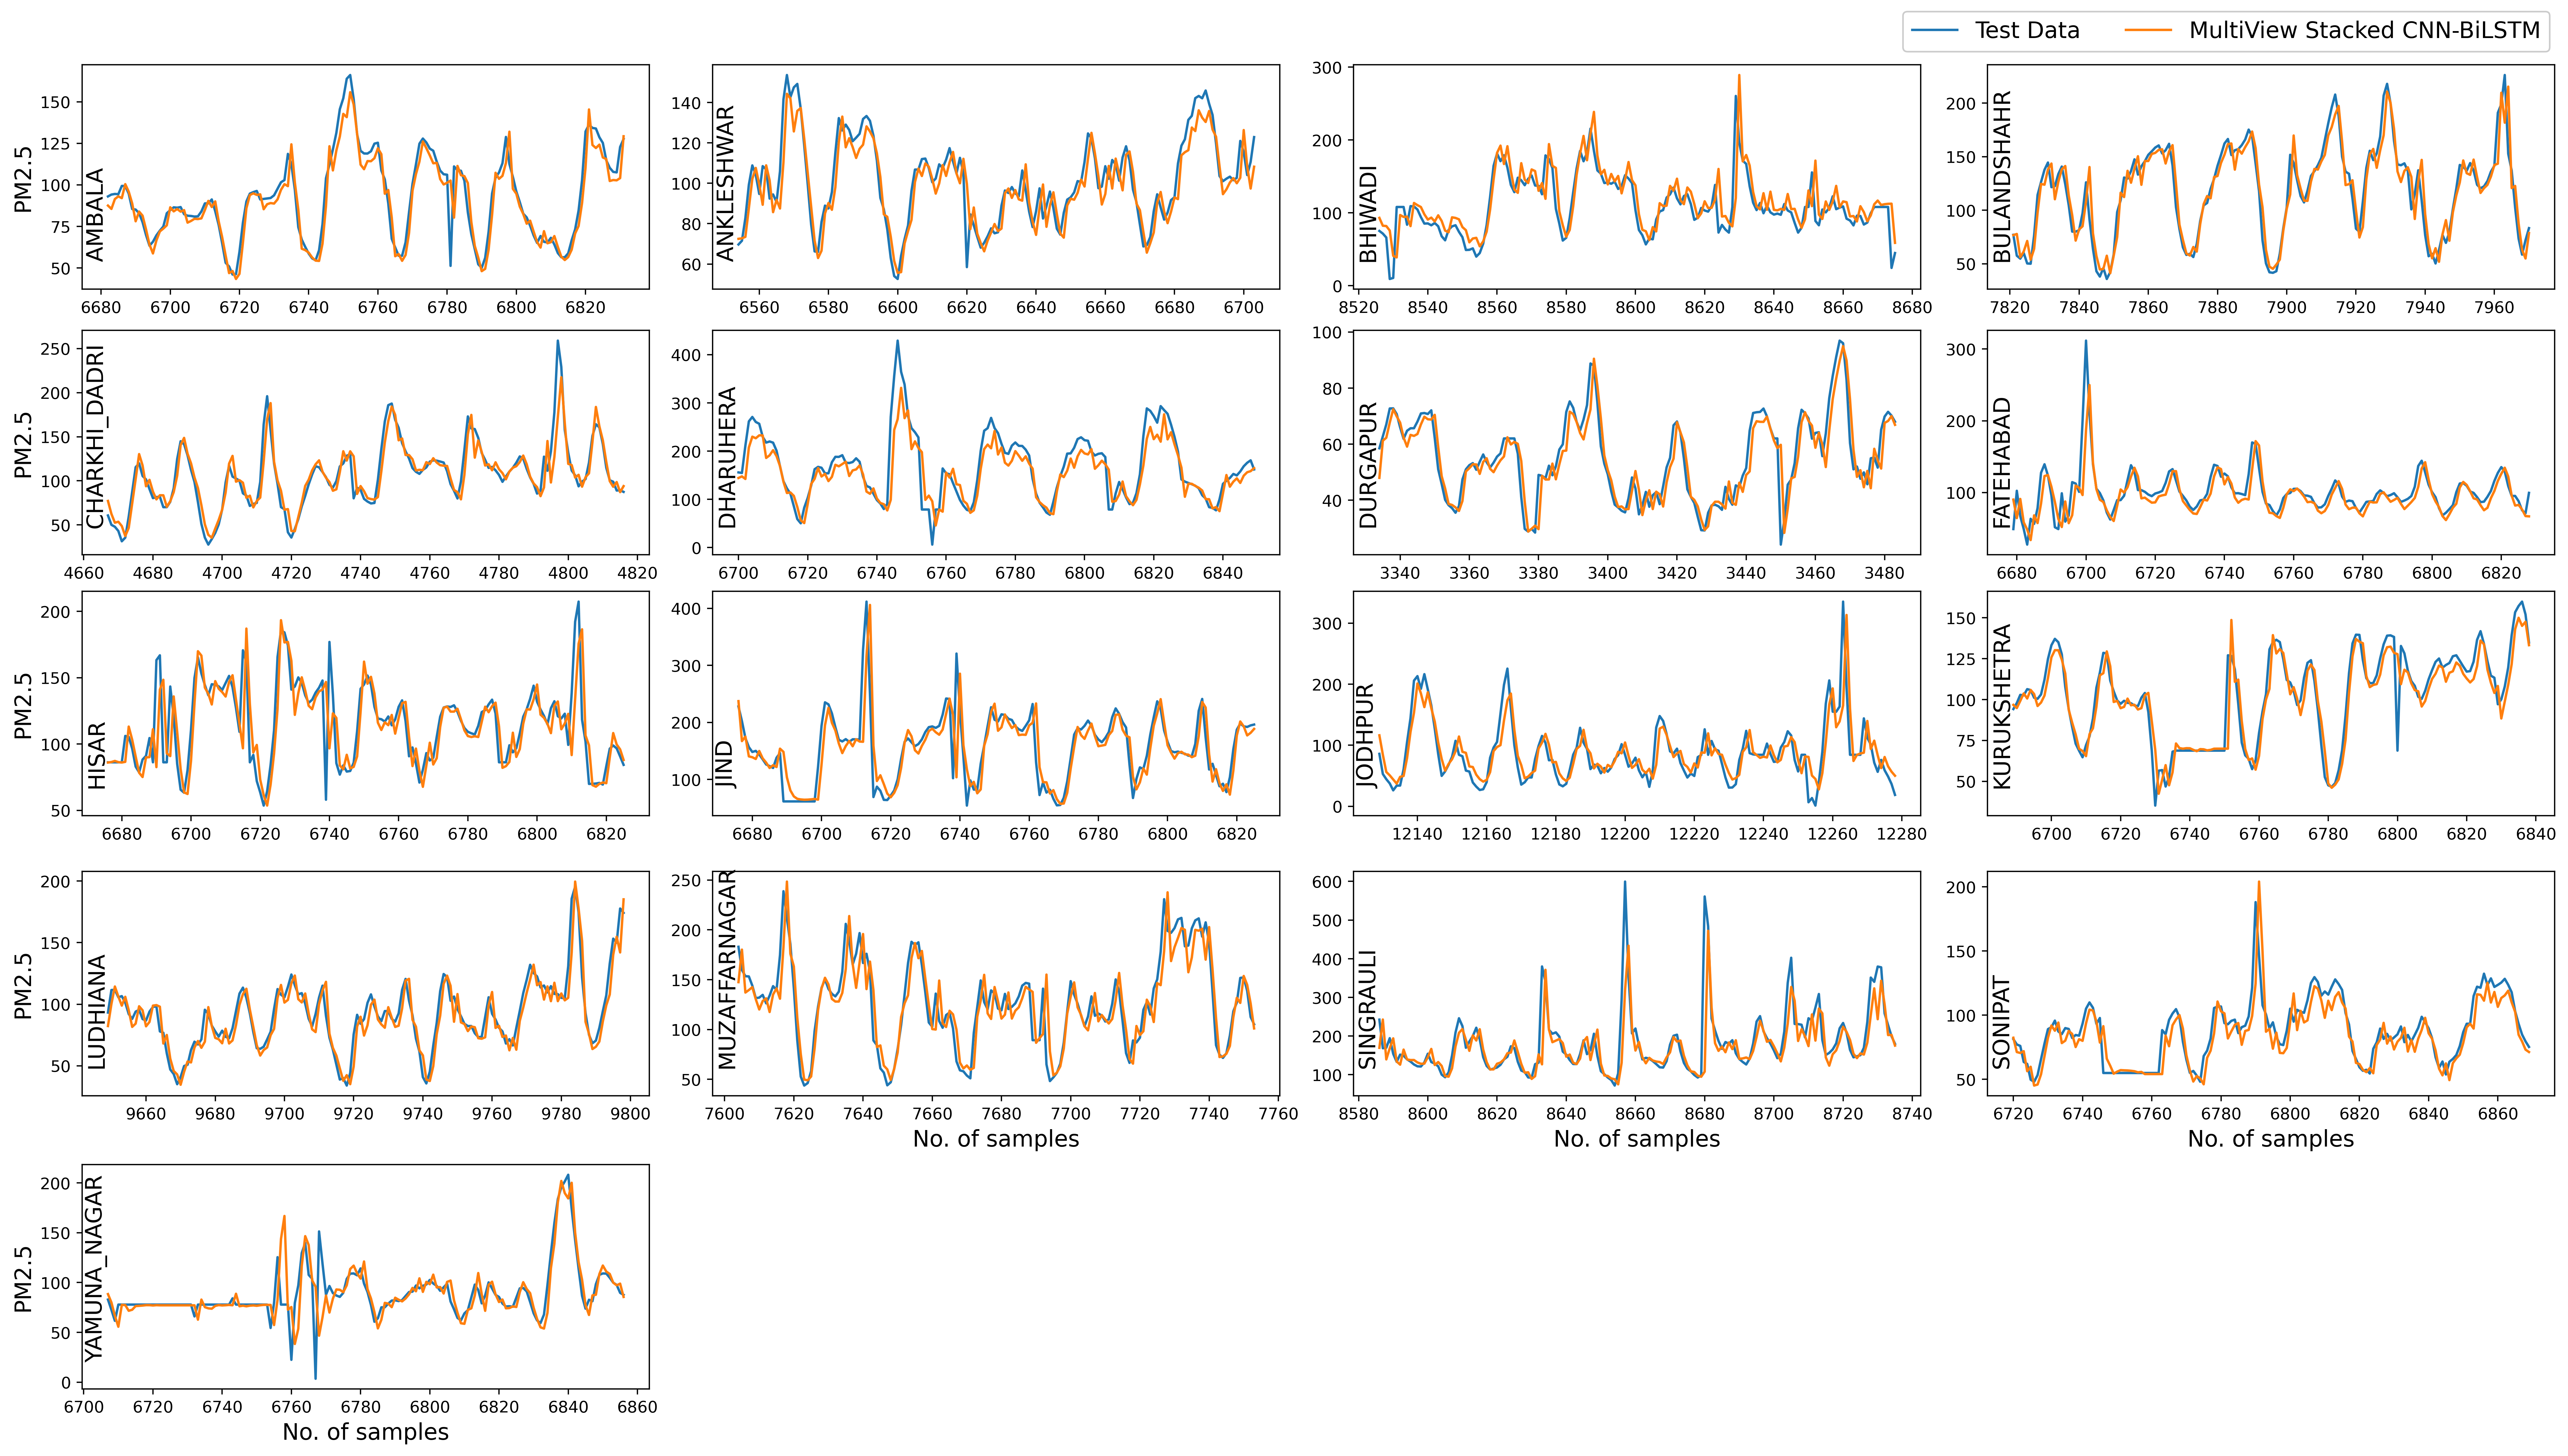
\includegraphics[scale=0.29]{img/act vs pri}
	  \caption{$PM_{2.5}$ predictions of proposed models MvS CNN-BiLSTM}\label{ACt_vs_Pred}
\end{figure*}
Figure \ref{ACt_vs_Pred} depicts a series of subplots that illustrate different datasets, each showcasing the comparison between the predicted and actual $PM_{2.5}$ values on the test dataset. The x-axis indicates the quantity of data points, while the $PM_{2.5}$ values are represented by the y-axis. Every subplot is associated with a specific dataset name, signifying the MvS CNN-BiLSTM model's evaluation performance on various datasets, which may reflect different time periods or locations where $PM_{2.5}$ concentrations were monitored and documented. In each subplot, the test dataset's individual samples are represented by data points. For each data point, there are two values plotted: the actual $PM_{2.5}$ value (ground truth) and the corresponding predicted $PM_{2.5}$ value generated by the MvS CNN-BiLSTM model. The plot allows us to visually compare how well the model's predictions match the actual values for each dataset.In Figure \ref{ACt_vs_Pred}, "prediction mimicking test" refers to the process of comparing the model's predicted values with the actual values in the test dataset to assess the accuracy and effectiveness of the predictive model.





% Please add the following required packages to your document preamble:
% \usepackage{graphicx}
\begin{table}[]
  \caption{RMSE Performance of traditional DL models and proposed models $($ MvS CNN-BiLSTM$)$.}
  \label{tab:RMSE}
  \resizebox{\textwidth}{!}{%
  \begin{tabular}{llllllcc}
 \hline DataSet        & BiLSTM  & CNN & GRU      & LSTM & RNN       & MvS CNN-BiLSTM        & Best-view \\ \hline
AMBALA         & 33.382          & 36.239    & \textbf{33.012} & 33.136     & 33.455                & 33.272          & 4      \\
ANKLESHWAR     & 22.916          & 23.724    & 22.975          & 23.359     & 22.807                & \textbf{22.081} & 6      \\
BHIWADI        & 28.043          & 25.168    & 25.521          & 26.512     & 25.974                & \textbf{24.959} & 10     \\
BULANDSHAHR    & 16.155          & 16.894    & \textbf{14.807} & 16.001     & 14.923                & 16.265          & 7      \\
 DCHARKHI\_DADRI & \textbf{30.071} & 32.709    & 32.299          & 32.629     & 33.836              & 31.064          & 3      \\
 DHARUHERA      & 25.751          & 26.948    & 26.057          & 26.108     & 25.489           &\textbf{24.983}          & 3      \\
 DURGAPUR       & 10.426          & 9.719     & 11.375          & 11.994     & 10.664                    & \textbf{8.906}  & 6      \\
 FATEHABAD      & 31.501          & 31.251    & 32.169          & 31.045     & 30.946                    & \textbf{30.86}  & 10     \\
 HISAR          & 21.677          & 22.286    & 20.875          & 21.371     & 21.617                 & \textbf{20.155} & 6      \\
 JIND           & 26.619          & 26.29     & 25.043          & 24.813     & \textbf{24.364}           & 24.408          & 10     \\
 JODHPUR        & 27.749          & 27.617    & 27.787          & 27.519     & 27.951              & \textbf{27.482} & 7      \\
 KURUKSHETRA    & 16.475          & 16.352    & 15.239          & 17.359     & \textbf{15.414}           & 15.921          & 5      \\
 LUDHIANA       & 14.573          & 17.013    & \textbf{13.817} & 17.668     & 14.936                    & 14.315          & 9      \\
 MUZAFFARNAGAR  & 20.885          & 23.182    & 21.206          & 20.412     & 23.638                   & \textbf{19.859} & 10     \\
 SINGRAULI      & 33.995          & 36.569    & \textbf{32.993} & 33.142     & 35.572                    & 33.834          & 2      \\
 SONIPAT        & 13.644          & 13.951    & 14.025          & 13.773     & 13.755                    & \textbf{12.75}  & 5      \\
 YAMUNA\_NAGAR  & 31.985          & 36.433    & 32.413          & 32.699     & 35.591                    & \textbf{31.676} & 8     \\ \hline
  \end{tabular}%
  }
  \end{table}
  Table \ref{tab:RMSE} exhibits the RMSE performance of different conventional DL models and the proposed MvS CNN-BiLSTM model on 17 datasets. The graph emphasizes the random-performing model (i.e., the model with unpredictable RMSE) for each dataset using strikethrough text. The leftmost column lists the names of the evaluated datasets, while the next columns represent the RMSE values of different traditional DL models on each dataset. The proposed MvS CNN-BiLSTM model's RMSE values are displayed in the "MvS CNN-BiLSTM" column. The "Best-view" column identifies the DL model that achieved the lowest RMSE on each dataset, highlighted using bold text.

  The table displays a thorough comparison of various DL models' RMSE performance across multiple datasets, with the MvS CNN-BiLSTM model demonstrating better RMSE values in its respective column and the bolded values indicating the best-performing model for each dataset.
  
  Table \ref{tab:RMSE} provides valuable insights into the predictive capabilities of traditional DL models and the proposed MvS CNN-BiLSTM model. The MvS CNN-BiLSTM model's for better performance over several traditional deep learning models on diverse datasets, as evidenced by the lower RMSE values. The highlighted values help identify the best model for each dataset, highlighting the effectiveness of the proposed MvS CNN-BiLSTM approach over traditional DL models.


  \begin{table}[]
    \caption{Percentage of improvement from MvS CNN-BiLSTM in RMSE}
    \label{RMSE imp}
    \begin{tabular}{llllcc}
    \hline    Dataset        &   BiLSTM &   CNN &   GRU &   LSTM &   RNN \\ \hline
    AMBALA         & 0.33 \%           & 8.19\%         & -0.79 \%       & -0.41 \%         & 0.55 \%            \\
    ANKLESHWAR     & 3.64  \%            & 6.93 \%        & 3.89 \%        & 5.47 \%         & 3.18 \%              \\
    BHIWADI       & 11.0  \%            & 0.83 \%         & 2.2 \%         & 5.86  \%        & 3.91 \%            \\
    BULANDSHAHR    & -0.68  \%            & 3.72 \%         & -9.85 \%       & -1.65  \%       & -8.99 \%               \\
    CHARKHI\_DADRI & -3.3 \%            & 5.03 \%        & 3.82 \%        & 4.8   \%        & 8.19   \%              \\
    DHARUHERA      & 2.98 \%            & 7.29 \%        & 4.12 \%        & 4.31 \%         & 1.99     \%             \\
    DURGAPUR       & 14.58 \%          & 8.37 \%         & 21.71 \%       & 25.75  \%       & 16.49  \%                \\
    FATEHABAD    & 2.03 \%           & 1.25 \%        & 4.07 \%        & 0.6    \%       & 0.28  \%                   \\
    HISAR          & 7.02 \%           & 9.56 \%        & 3.45 \%        & 5.69  \%        & 6.76  \%                   \\
    JIND           & 8.31 \%           & 7.16 \%        & 2.54 \%        & 1.63 \%         & -0.18 \%                    \\
    JODHPUR        & 0.96 \%           & 0.49 \%         & 1.1 \%         & 0.13 \%          & 1.68 \%                     \\
    KURUKSHETRA    & 3.36 \%           & 2.64 \%        & -4.48  \%      & 8.28 \%         & -3.29  \%                 \\
    LUDHIANA      & 1.77 \%           & 15.86 \%       & -3.6  \%       & 18.98 \%      & 4.16   \%                  \\
    MUZAFFARNAGAR  & 4.91 \%           & 14.33 \%       & 6.35 \%         & 2.71 \%         & 15.99 \%                    \\
    SINGRAULI      & 0.47 \%           & 7.48 \%        & -2.55 \%       & -2.09 \%        & 4.89  \%                   \\
    SONIPAT        & 6.55 \%           & 8.61 \%        & 9.09 \%        & 7.43 \%         & 7.31  \%                    \\
    YAMUNA\_NAGAR  & 0.97 \%           & 13.06 \%       & 2.27 \%        & 3.13 \%         & 11.0  \%                   \\ \hline
    \end{tabular}
    \end{table}
    Table \ref{RMSE imp} illustrates the extent $\%$ of improvement from conventional deep learning (DL) models to the proposed MvS CNN-BiLSTM model across 17 datasets. The chart showcases the growth rate of every deep learning model, namely BiLSTM, CNN, GRU, LSTM, and RNN, with respect to the MvS CNN-BiLSTM model. Negative values indicate that the corresponding DL model outperformed the MvS CNN-BiLSTM model for a particular dataset. The table consists of a pair of columns that are connected. The right column depicts the percentage of regression for the multivariate effective CNN-BLSTM model in comparison to traditional DL models for each dataset evaluated in the study in the left column. For each dataset, the corresponding percentage of improvement for each DL model is presented in their respective columns. A positive percentage value denotes that the MvS CNN-BiLSTM model performed better than the specific DL model by the percentage indicated.
   \begin{comment}  A negative percentage value signifies that the specific DL model outperformed the MvS CNN-BiLSTM model by the percentage indicated. In summary, Table \ref{RMSE imp} provides a quantitative measure of the improvement achieved by the proposed MvS CNN-BiLSTM model over traditional DL models. Positive values serve as evidence of MvS CNN-BiLSTM model's superiority over conventional DL models, whereas negative values indicate better performance of certain traditional DL models for specific datasets. The table, as a whole, affirms the potency of the proposed MvS CNN-BiLSTM model by showcasing its exceptional performance on most datasets in contrast to traditional DL models.
   \end{comment}


\begin{table}[!htp]
  \caption{Average Rankings of the algorithms (Friedman) in contest of RMSE}
  \centering
  \begin{tabular}{lccc}
  \hline
  Algorithm&Ranking&$p$&Holm\\\hline
  BiLSTM&3.7059&0.002485&0.016667\\
  CNN&4.8235&0.000002&0.01\\
  GRU&3.1765&0.027801&0.05\\
  LSTM&3.8235&0.001335&0.0125\\
  RNN&3.7059&0.002485&0.025\\
  \textbf{MvS CNN-BiLSTM}&\textbf{1.7647}&$-$ &$-$ \\\hline
\end{tabular}
\label{rank_rmse}
  \end{table}
  Table \ref{rank_rmse} exhibits the average rankings of various algorithms in relation to the RMSE metric, thereby providing insights into their relative performance. The table comprises four columns, viz. algorithm, Ranking, $p$-value, and Holm. The names of several algorithms, including BiLSTM, CNN, GRU, LSTM, RNN, and the recently suggested MvS CNN-BiLSTM, are being logged in the algorithm column while the assessment process is underway. The standing column exhibits the mean ranks of every algorithm relying on their performance in terms of RMSE, where a lesser rank indicates superior performance with 1 being the best rank and higher numbers indicating weaker performance. Each algorithm's comparison is assigned a significance level in the $p$-value column, with a small $p$-value indicating a statistically significant difference in performance between the compared algorithms. The Holm column serves the purpose of controlling the family-wise error rate by indicating adjusted significance thresholds utilized in multiple statistical tests. The parposed MvS CNN-BiLSTM algorithm accomplished an average ranking of 1.7647, which is the finest among all compared models with respect to RMSE. The MvS CNN-BiLSTM algorithm was not used in the given comparison of traditional shallow learning models (BiLSTM, CNN, GRU, LSTM, and RNN). Furthermore, the minute $p$-values for every algorithmic comparison imply a statistically significant variance in performance amongst all the algorithms, signifying that the performance of each algorithm is discernible from others based on the RMSE metric. The Holm column likely indicates the adjusted significance thresholds (critical values) used in the Holm method for multiple comparisons, which is a statistical procedure used to control the family-wise error rate when performing multiple hypothesis tests. The MvS CNN-BiLSTM algorithm is the superior choice based on the table's data, performing better than other algorithms in RMSE.








% Please add the following required packages to your document preamble:
% \usepackage{graphicx}
\begin{table}[]
  \caption{MAPE Performance of traditional DL models and proposed models $($MvS CNN-BiLSTM$)$}
  \label{tab:MAPE}
  \resizebox{\textwidth}{!}{%
  \begin{tabular}{llllllcc}
 \hline DataSet        & BiLSTM  & CNN & GRU      & LSTM & RNN      & MvS CNN-BiLSTM        & Best-view \\ \hline
  AMBALA         & 54.468       & 49.153    & 76.839    & 58.619     & 53.375    & \textbf{18.73}  & 3      \\
  ANKLESHWAR     & 18.86        & 19.968    & 19.015    & 19.576     & 20.72     & \textbf{16.265} & 10     \\
  BHIWADI        & 134.448      & 118.741   & 123.123   & 127.481    & 124.503   & \textbf{20.98}  & 2      \\
  BULANDSHAHR    & 44.602       & 47.066    & 26.254    & 43.721     & 27.813    & \textbf{22.469} & 3      \\
  CHARKHI\_DADRI & 50.328       & 101.385   & 102.063   & 112.912    & 115.673   & \textbf{26.728} & 10     \\
  DHARUHERA      & 35.638       & 39.358    & 39.557    & 35.942     & 40.34     & \textbf{17.365} & 3      \\
  DURGAPUR       & 45.511       & 37.529    & 56.324    & 57.457     & 48.626    & \textbf{19.321} & 6      \\
  FATEHABAD      & 19.737       & 19.929    & 19.475    & 18.663     & 17.724    & \textbf{12.178} & 5      \\
  HISAR          & 17.971       & 18.422    & 17.988    & 17.983     & 21.475    & \textbf{15.082} & 6      \\
  JIND           & 25.945       & 30.822    & 27.344    & 24.596     & 33.464    & \textbf{16.618} & 3      \\
  JODHPUR        & 40.188       & 40.36     & 41.584    & 41.578     & 43.36     & \textbf{28.278} & 7      \\
  KURUKSHETRA    & 13.713       & 13.392    & 12.405    & 13.986     & 13.312    & \textbf{11.248} & 2      \\
  LUDHIANA       & 37.61        & 47.14     & 34.504    & 51.036     & 41.197    & \textbf{15.706} & 9      \\
  MUZAFFARNAGAR  & 24.162       & 27.253    & 23.37     & 26.08      & 27.061    & \textbf{16.571} & 5      \\
  SINGRAULI      & 48.642       & 67.143    & 39.738    & 34.372     & 68.525    & \textbf{28.545} & 7      \\
  SONIPAT        & 43.301       & 48.32     & 49.409    & 43.187     & 45.67     & \textbf{13.541} & 7      \\
  YAMUNA\_NAGAR  & 65.601       & 63.698    & 64.637    & 63.404     & 70.02     & \textbf{28.29}  & 10    \\ \hline
  \end{tabular}%
  }
  \end{table}
Table \ref{tab:MAPE} showcases MAPE results of the MvS CNN-BiLSTM model and traditional DL models across 17 datasets. The DL models analyzed in the table include BiLSTM, CNN, GRU, LSTM, and RNN. The MAPE values for each DL model are compared with those of the MvS CNN-BiLSTM model. The minimum MAPE values obtained by each model for each dataset, along with the corresponding best view, are presented in \textbf{bold}. To expound the Table \ref{tab:MAPE}, the initial column enumerates the names of the datasets assessed in the investigation. The succeeding columns indicate the MAPE values for the different traditional DL models compared to the proposed MvS CNN-BiLSTM model for each dataset. The table's interpretation involves the presentation of the corresponding MAPE value for each DL model to their respective columns. The "Best-view" column, on the other hand, specifies the best dataset for which the MvS CNN-BiLSTM model obtained the minimum MAPE value. In conclusion, Table \ref{tab:MAPE} offers a thorough comparison of the MAPE performance of the MvS CNN-BiLSTM model and traditional DL models across multiple datasets. The values in \textbf{bold} highlight the MvS CNN-BiLSTM model's superior performance over traditional DL models for different datasets. The table demonstrates the MvS CNN-BiLSTM model's ability to reduce MAPE for air quality prediction in various locations and datasets.

  \begin{table}[]
    \caption{Improvement from MvS CNN-BiLSTM in MAPE}
    \label{MAPE imp}
    \begin{tabular}{lllcc}
    \hline   Dataset       &   BiLSTM &   GRU &   LSTM &   RNN  \\ \hline
      AMBALA        &35.74           \% &58.11        \% &39.89         \% &34.64 \%       \\
      ANKLESHWAR      &2.59            \% &2.75         \% &3.31          \% &4.45 \%          \\
      BHIWADI        &113.47          \% &102.14       \% &106.5         \% &103.52 \%        \\
      BULANDSHAHR   &22.13           \% &3.78         \% &21.25         \% &5.34   \%        \\
      CHARKHI\_DADRI  &23.6            \% &75.34        \% &86.18         \% &88.94 \%         \\
      DHARUHERA      &18.27           \% &22.19        \% &18.58         \% &22.98 \%         \\
      DURGAPUR       &26.19           \% &37.0         \% &38.14         \% &29.3 \%          \\
      FATEHABAD       &7.56            \% &7.3          \% &6.48          \% &5.55 \%           \\
      HISAR           &2.89            \% &2.91         \% &2.9           \% &6.39 \%          \\
      JIND            &9.33            \% &10.73        \% &7.98          \% &16.85 \%         \\
      JODHPUR         &11.91           \% &13.31        \% &13.3          \% &15.08 \%          \\
      KURUKSHETRA     &2.46            \% &1.16         \% &2.74          \% &2.06 \%          \\
      LUDHIANA        &21.9            \% &18.8         \% &35.33         \% &25.49 \%         \\
      MUZAFFARNAGAR   &7.59            \% &6.8          \% &9.51          \% &10.49 \%          \\
      SINGRAULI      &20.1            \% &11.19        \% &5.83          \% &39.98 \%         \\
      SONIPAT        &29.76           \% &35.87        \% &29.65         \% &32.13 \%         \\
      YAMUNA\_NAGAR   &37.31           \% &36.35        \% &35.11         \% &41.73 \%         \\ \hline
    \end{tabular}
    \end{table}
    Table \ref{MAPE imp} displays the percentage improvement in MAPE attained by the proposed MvS CNN-BiLSTM model in comparison to various traditional DL models (BiLSTM, GRU, LSTM, RNN) for all 17 datasets. The first column of the table lists the names of the datasets evaluated in the study. The succeeding columns represent the percentage improvement in MAPE achieved by the MvS CNN-BiLSTM model over each traditional DL model on each dataset. The percentage values in the table indicate the reduction in MAPE attained by the MvS CNN-BiLSTM model relative to each traditional DL model, with negative values implying cases where the traditional DL model outperformed the MvS CNN-BiLSTM model.
\begin{comment}
    In summary, Table \ref{MAPE imp} provides a comprehensive overview of the advancement in MAPE achieved by the proposed MvS CNN-BiLSTM model compared to traditional DL models for diverse datasets. Positive percentage values signify that the MvS CNN-BiLSTM model performed better, while negative values suggest that the traditional DL model performed better. Overall, the table emphasizes the superiority of the proposed model in reducing MAPE and enhancing air quality prediction accuracy across different datasets and locations.
\end{comment}

    \begin{table}[!htp]
      \caption{Average rankings of the algorithms (Friedman) in contex of MAPE}
      \centering
      \begin{tabular}{lccc}\hline
      Algorithm&Ranking&$p$&Holm\\\hline
      BiLSTM&3.4706&0.000118&0.05\\
      CNN&4.1765&0.000001&0.0125\\
      GRU&3.7647&0.000016&0.025\\
      LSTM&3.8824&0.000007&0.016667\\
      RNN&4.7059&0&0.01\\
      \textbf{MvS CNN-BiLSTM}&\textbf{1}&$-$ &$-$\\\hline
    \end{tabular}
      
      \label{rank_mape}
      \end{table}
      Table \ref{rank_mape} showcases the average rankings of multiple algorithms in the context of the MAPE metric, providing insight into the relative performance of these algorithms. The primary row comprises the appellation of the systems being measured, particularly BiLSTM, CNN, GRU, LSTM, RNN, and the parposd MvS CNN-BiLSTM. The subsequent column displays the average rankings of each algorithm according to their MAPE performance, with a lower ranking indicating superior performance, and a greater number indicating inferior performance. The third column denotes the p-values which is the level of significance for comparing each algorithm. A statistically significant difference in performance between the compared algorithms is present if the $p$-value is low. The fourth column, "Holm," is likely to denote the critical values or adjusted significance thresholds used for multiple comparisons. The Holm method is used to manage the family-wise error rate when conducting multiple statistical tests.
      
      The MvS CNN-BiLSTM algorithm is better in terms of MAPE, surpassing all other models, including BiLSTM, CNN, GRU, LSTM, and RNN, with an average rank of 1. It is thus improbable to assume that any other compared algorithm outperforms the MvS CNN-BiLSTM algorithm in terms of MAPE. Furthermore, the small $p$-values for every algorithmic comparison indicate that there are statistically significant disparities in efficacy among all of the algorithms. This implies that the algorithms' performance is distinguishable from one another based on the MAPE metric. As for the "Holm" column, it likely denotes the adjusted significance thresholds (critical values) used in the Holm method for multiple comparisons.The Holm method is a statistical technique employed for controlling family-wise error rate during the execution of multiple hypothesis tests. In summary, Table \ref{rank_mape} show that the proposed MvS CNN-BiLSTM algorithm is the best among all the compared algorithms in terms of MAPE. Moreover, there exist statistically meaningful distinctions in performance among the MAPE metric-based algorithms.
    



% Figure
\begin{figure}[ht]
	\centering
		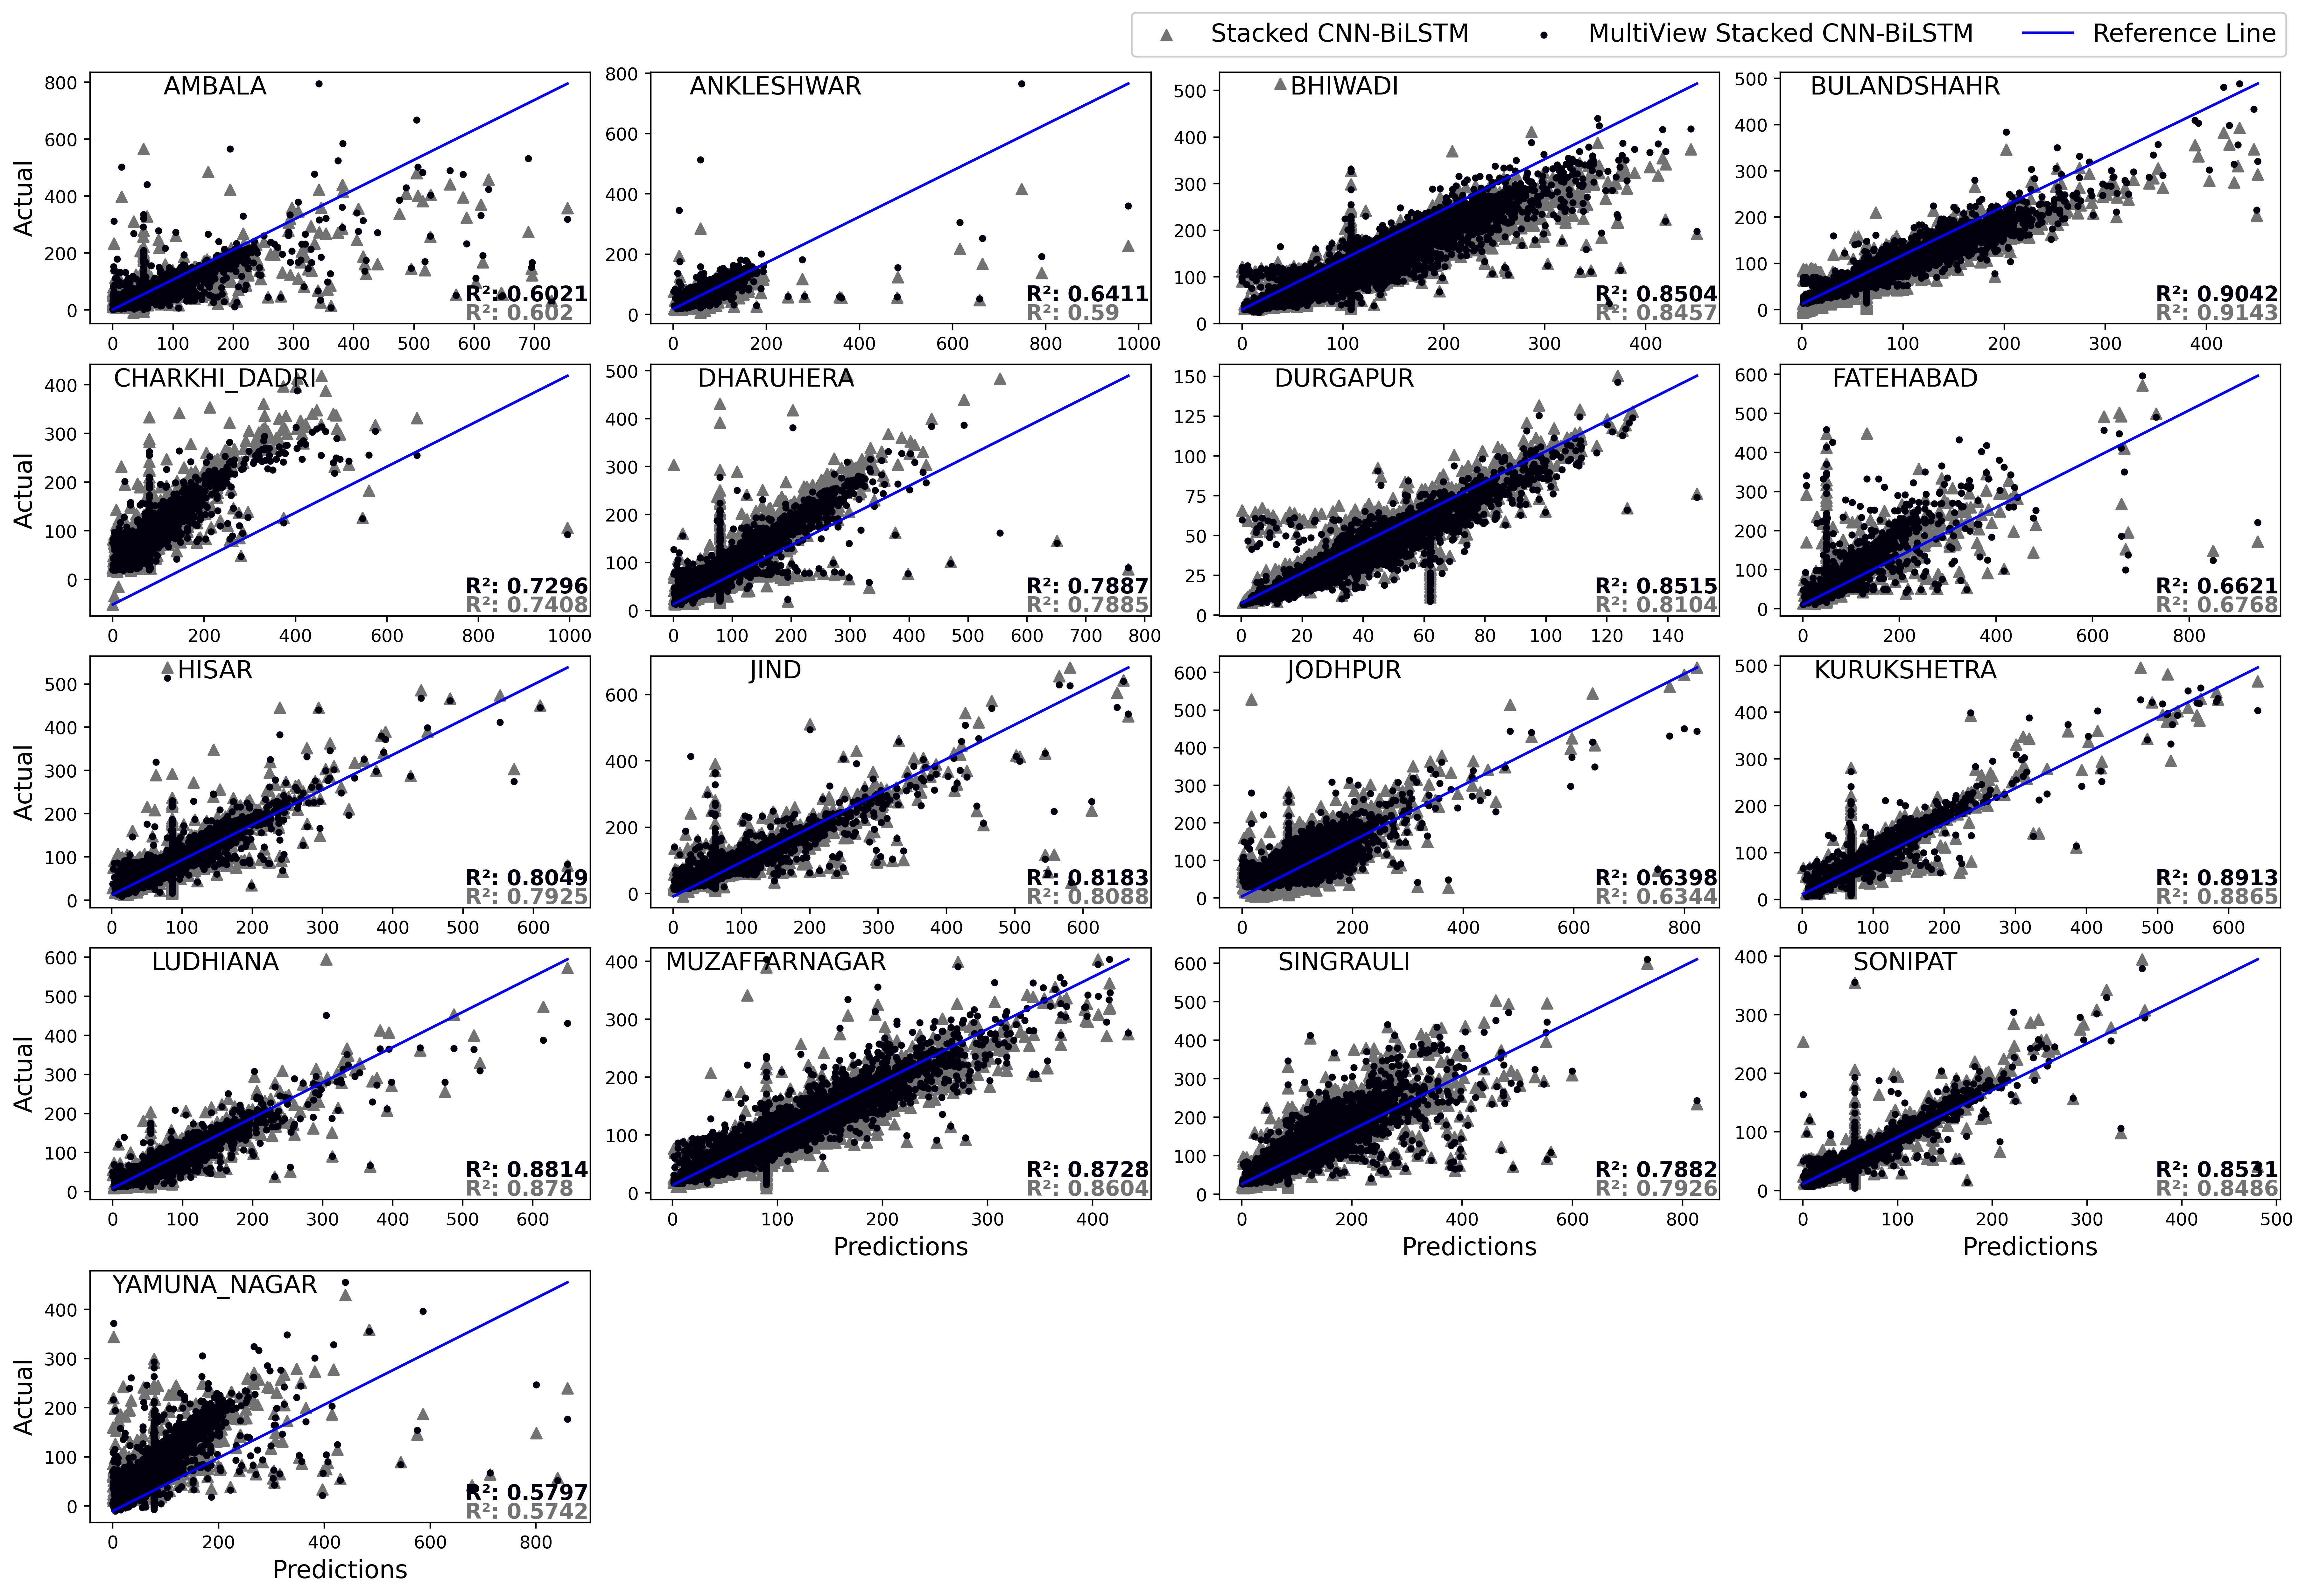
\includegraphics[scale=0.35]{img/Scatter_plot}
	  \caption{Correlation of Actual values and Predictions of proposed models $($Stacked CNN-BiLSTM and MvS CNN-BiLSTM $)$ using Scatter plot.}\label{Scatter}
\end{figure}
The Figure \ref{Scatter} contains 17 subplots, each of which displays a scatter plot for multiple datasets, and compares the gray Stacked CNN-BiLSTM model with the black Proposed MvS CNN-BiLSTM model. The plot includes a blue reference line that represents the optimal scenario in which predicted and actual values are in complete alignment. Additionally, each subplot displays two $R^2$ values, corresponding to the gray and black superimposed plots. A heightened $R^2$ value suggests a more powerful correlation between anticipated and real values, making it a valuable statistical gauge of fitness in provided Figure, there are two potential interpretations: If the gray Stacked CNN-BiLSTM has a greater $R^2$ value than the black Proposed MvS CNN-BiLSTM, The analysis shows that the grey model had superior accuracy and a more resilient correlation between projected and actual values than the black model, leading to a superior overall fit. The same $R^2$ value of the black Proposed MvS CNN-BiLSTM and the gray Stacked CNN-BiLSTM makes it irrelevant which model performed better in predicting actual values and has a similar goodness-of-fit and correlation with actual values. Based on the information you provided, it appears that for the Figure \ref{Scatter} Singrauli, Fatehabad, Charkhi\_Dadri, and Bulandshahr, the gray Stacked CNN-BiLSTM model has higher $R^2$ values compared to the black Proposed MvS CNN-BiLSTM model. However, you mentioned that the $R^2$ values for the black model are very close to the gray model. In this case, since the $R^2$ values for the black model are very close to the gray model, it suggests that both models have similar predictive performance for those datasets. The difference in their $R^2$ values might be small, indicating that they are both relatively accurate in predicting the actual values. It has conclued that the assocition of multi-view leading with stacked CNN-BiLSTM is performing better than the stacked CNN-BiLSTM along with traditional model over varraus measures.


\begin{table}[!htp]
  \caption{Overall average of RMSE and MAPE ranking of traditional models and proposed model (MvS CNN-BiLSTM)}
  \centering
  \begin{tabular}{lccc}
  \hline
  Algorithm&RMSE\_Ranking&MAPE\_Ranking&Average\_Ranking\\\hline
  BiLSTM&3.7059&3.4706&3.58825\\
  CNN&4.8235&4.1765&4.5\\
  GRU&3.1765&3.7647&3.4706\\
  LSTM&3.8235&3.8824&3.85295\\
  RNN&3.7059&4.7059&4.2059\\
  \textbf{MvS CNN-BiLSTM}&\textbf{1.7647}&\textbf{1}&\textbf{1.38235} \\\hline
\end{tabular}
\label{AVG RANK}
  \end{table}



  \begin{figure*}[h!]
    \centering
    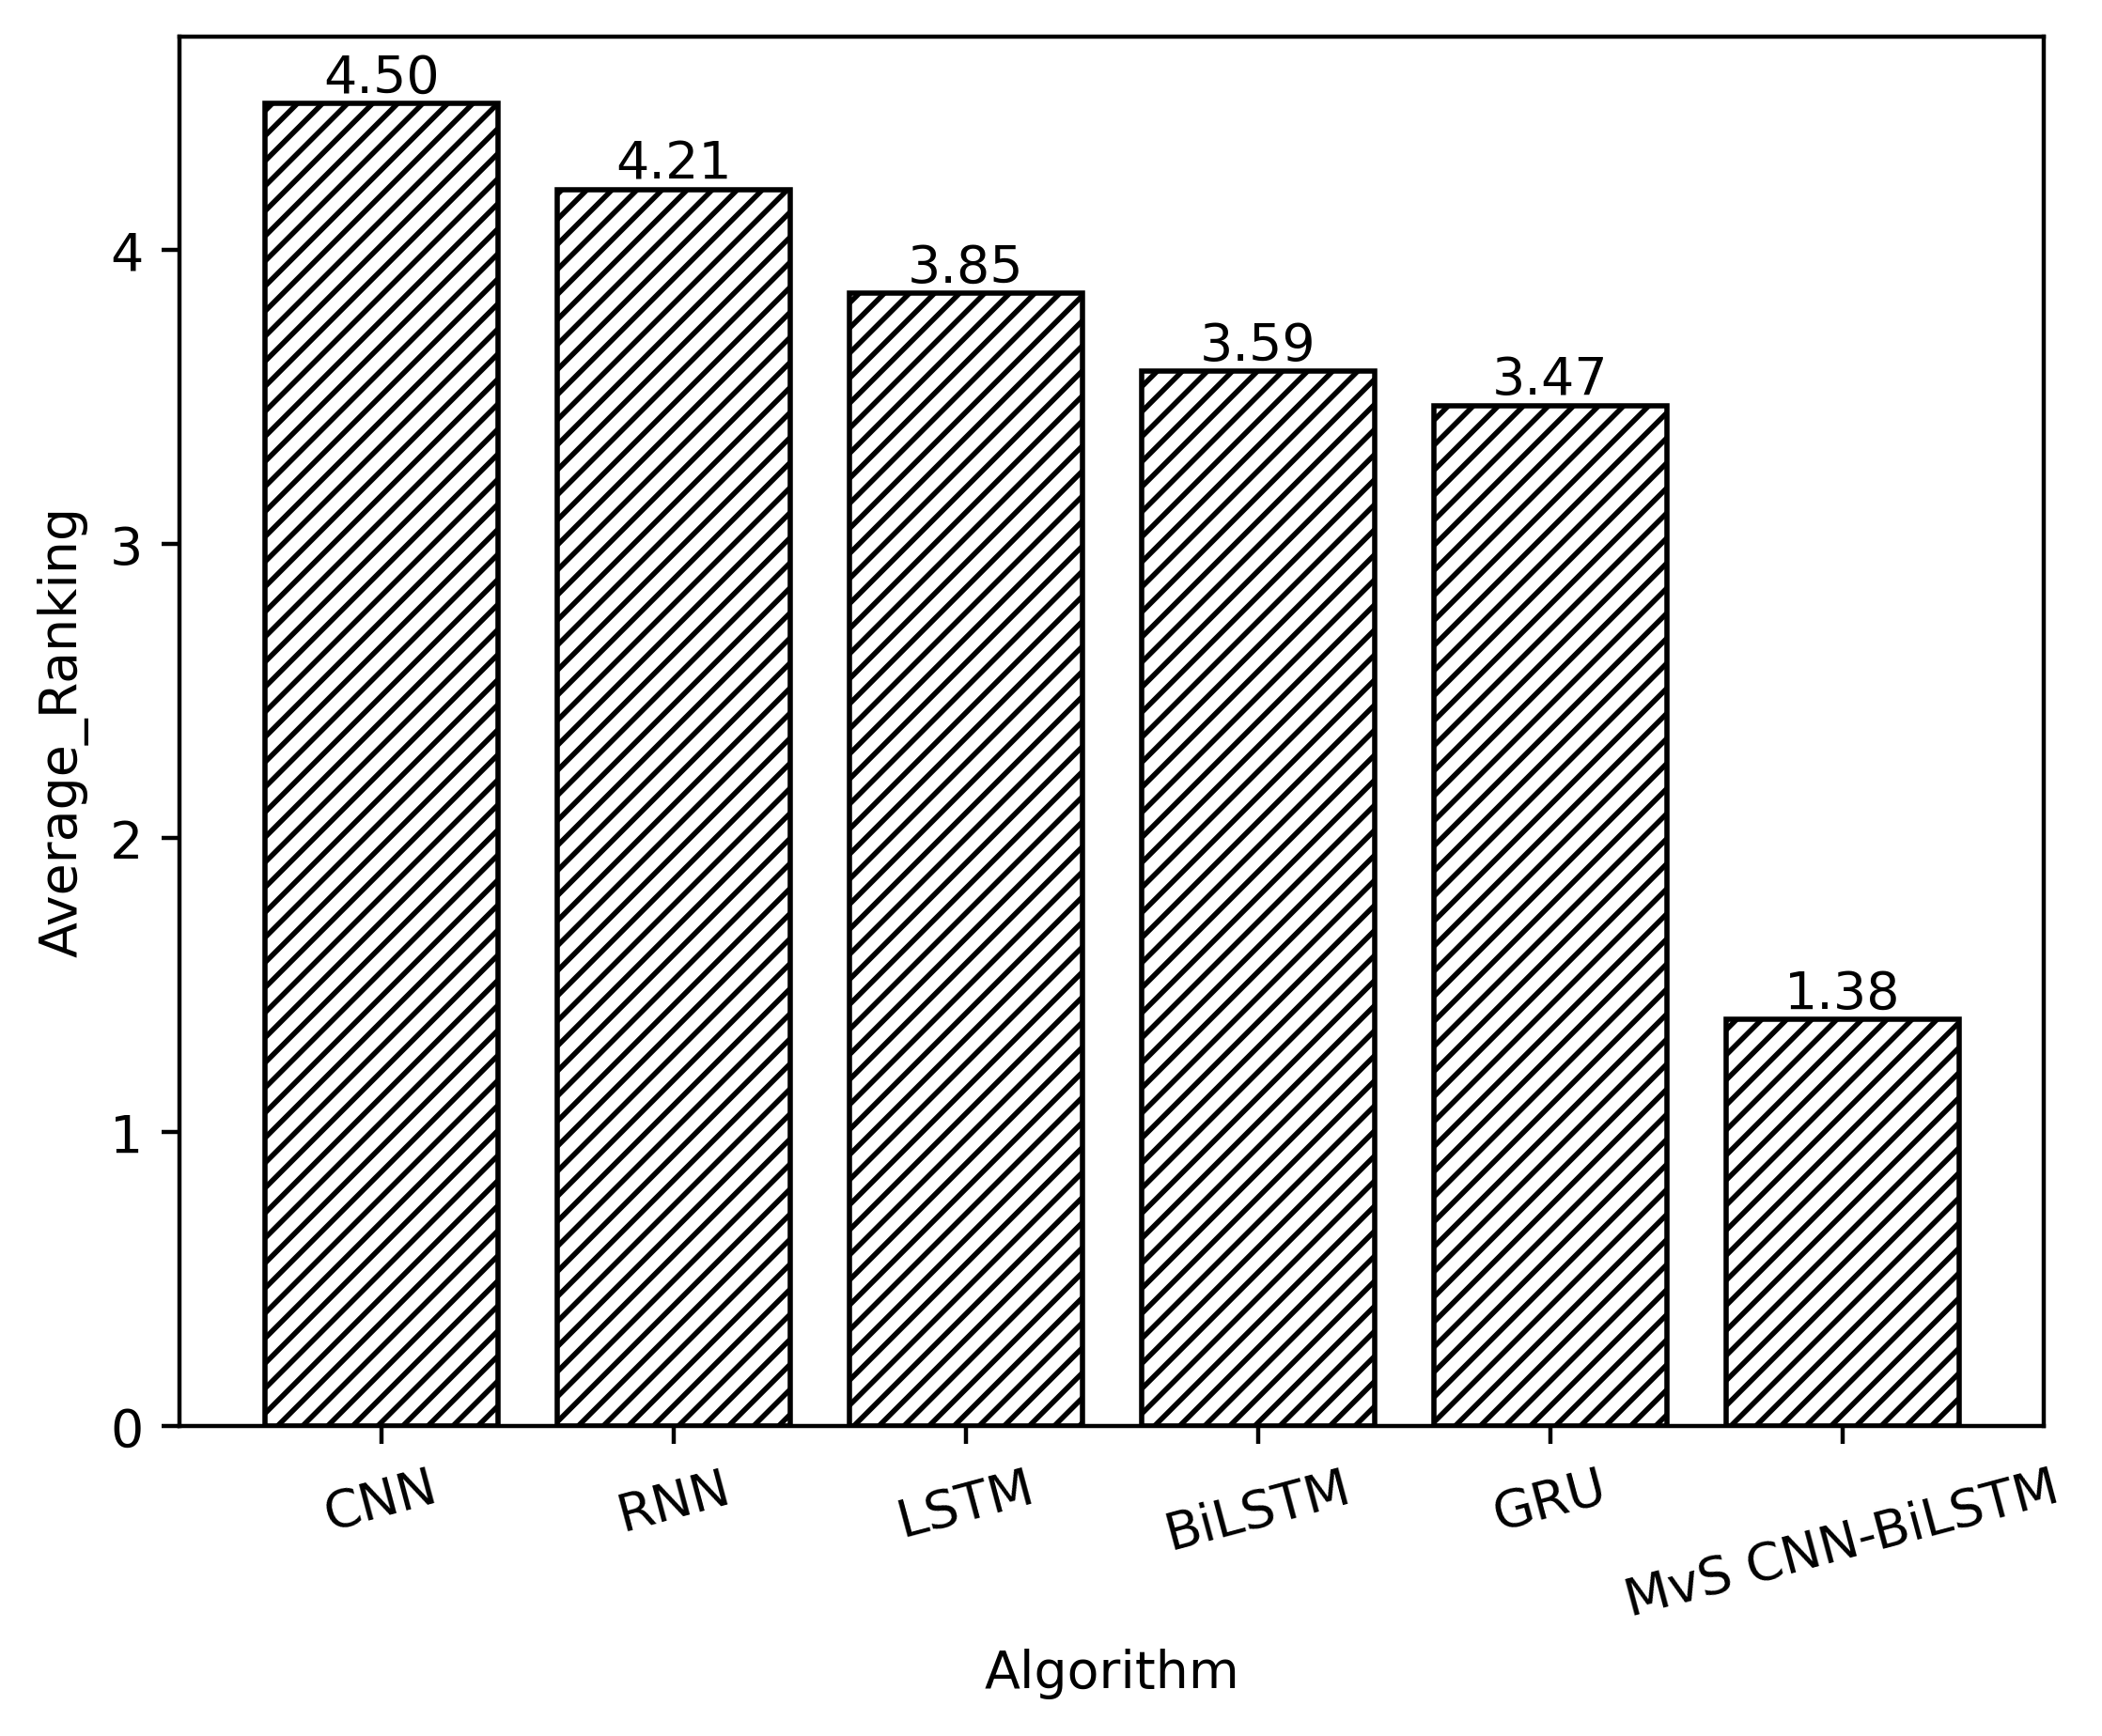
\includegraphics[scale=0.7]{img/avg_Rank_plot}
    \caption{Overall average Friedman ranking of traditional models and proposed MvS CNN-BiLSTM model.}
    \label{avg_Rank_plot}
  \end{figure*}
  In Table \ref{AVG RANK}, the mean rankings of various algorithms are presented according to their performance on two performance metrics, namely RMSE and MAPE. The table also includes an additional column for the average ranking across both metrics. The initial column suggests the average positions of each formula based on their RMSE performance, whereas the second column displays the average positions of each formula based on their MAPE performance. The third column signifies the mean rank of each algorithm, factoring in performance on both metrics and providing a comprehensive measure of performance. In Table \ref{AVG RANK} show avrage ranking on both praformance measures and conclued best algotitham on both measures. The underperformance of conventional deep learning structures such as BiLSTM, CNN, GRU, LSTM, and RNN, despite their higher ranking on average, is a surprising observation compared to the MvS CNN-BiLSTM method.Thus, according to Figure \ref{avg_Rank_plot} the mean ranking over the two performance metrics, the MvS CNN-BiLSTM algorithm is regarded as the optimal algorithm out of all the models.The bar graph provided is illegible and cannot be used to support the previous analysis, showing that the MvS CNN-BiLSTM algorithm has no ranking or comparison to the traditional deep learning models (BiLSTM, CNN, GRU, LSTM, and RNN) on average for the given task. The CNN and RNN algorithms were actually rated the worst on average, suggesting that their performance was not as great as other models.

\begin{comment} It is improbable that any other algorithm can surpass the proposed MvS CNN-BiLSTM algorithm's remarkable performance, which achieved the best average ranking of 1.38235 based on the average rankings across both RMSE and MAPE metrics.\end{comment}



\section{Conclusions}
Our findings from analyzing the forecasting of $PM_{2.5}$ levels in Indian cities using deep learning techniques have led us to a number of conclusions. The suggested MvS CNN-BiLSTM methods have been proven to be effective tools for predicting Indian city $PM_{2.5}$ levels. The implementation of intricate training models has furnished optimistic findings, implying that they boast the potential to considerably augment air quality projections. It should be noted, nonetheless, that the performance of these models is reliant on the specific city and season. Some locations may produce more precise forecasts than others, highlighting the importance of customizing the models to different geographical regions and seasons.


\section*{CRediT authorship contribution statement}

\section*{Data availability}
Data will be available on \href{https://app.cpcbccr.com/ccr/#/caaqm-dashboard-all/caaqm-landing}{CPCB(India)} Webportel.The \href{https://www.cpcb.nic.in/}{Central Pollution Control Board (CPCB) } in India maintains a web portal that offers access to various environmental datasets, including air and water quality, emission inventories, and pollution monitoring data, aimed at promoting environmental awareness and research in the country.
\section*{Acknowledgments}
We extend our heartfelt appreciation to the Central Pollution Control Board (CPCB), India, for generously providing invaluable environmental data, which significantly enhanced our research and played a pivotal role in the successful completion of this study.
\label{}

% Numbered list
% Use the style of numbering in square brackets.
% If nothing is used, default style will be taken.
%\begin{enumerate}[a)%\item 
%\item 
%\item 
%\end{enumerate}  

% Unnumbered list
%\begin{itemize}
%\item 
%\item 
%\item 
%\end{itemize}  

% Description list
%\begin{description}
%\item[]
%\item[] 
%\item[] 
%\end{description}  


\begin{comment}

\begin{table}[<options>]
\caption{}\label{tbl1}
\begin{tabular*}{\tblwidth}{@{}LL@{}}
\toprule
 & \\ % Table header row
\midrule
 & \\
 & \\
 & \\
 & \\
\bottomrule
\end{tabular*}
\end{table}



\end{comment}
% Uncomment and use as the case may be
%\begin{theorem} 
%\end{theorem}

% Uncomment and use as the case may be
%\begin{lemma} 
%\end{lemma}

%% The Appendices part is started with the command \appendix;
%% appendix sections are then done as normal sections
%% \appendix




\label{}

% To print the credit authorship contribution details
\printcredits

%% Loading bibliography style file
%\bibliographystyle{model1-num-names}
\bibliographystyle{cas-model2-names}

% Loading bibliography database
\bibliography{ref}

% Biography
\bio{}
% Here goes the biography details.
\endbio

%\bio{pic1}
% Here goes the biography details.
\endbio

\end{document}

